% !TEX root = ../thesis-example.tex
%
\chapter{Interface sensible / hardware}
\label{ch:interfaces}

\cleanchapterquote{Komponieren heißt: über die Mittel nachdenken.\\
Komponieren heißt: ein Instrument bauen.\\
Komponieren heißt: nicht sich gehen,\\
sondern sich kommen lassen.}
{Helmut Lachenmann}{1986}

\cleanchapterquote{Fingers are not to be despised:\\
they are great inspirers, and,\\
in contact with a musical instrument,\\
often give birth to subconscious ideas \\
which might otherwise never come to life.}
{Igor Stravinsky}{1936}

\noindent Dans ce chapitre sont étudiés un certain nombre de d'aspects de la part matérielle des \glspl{DMI}. Parallèlement seront présentées deux interfaces que j'ai développées pour ma pratique musicale : le Filigramophone (figure \ref{fig:interface:filigramophone_unplugged}) et le Xypre (figure \ref{fig:interface:xypre_unplugged}). Ces deux interfaces sont en quelque sorte des variations sur un même archétype d'instrument ``tablette'', né de l'utilisation initiale d'une tablette graphique Wacom. Leur design reflète les différentes contraintes rencontrées lors du passage d'une technologie à une autre et comment un même modèle général d'interaction est adapté en fonction du medium et des technologies qui l'implémente et l'incarne.

Il faut ici rappeler que les \glspl{DMI}, s'ils se caractérisent par l'usage de la computation numérique, sont aussi nécessairement des instruments électroniques, électriques et acoustiques. Il portent l'héritage et les contraintes propres à ces différents médias.

%------------ Figure : filigramophone et xypre -----------
\begin{figure}[!htbp]
	\captionsetup{format=plain}%
	\centering
	\begin{minipage}[t]{0.48\textwidth}
		
\includegraphics[width=\linewidth]{gfx/dummy.pdf}
		\caption[Filigramophone: vue d'ensemble]{TODO : Filigramophone, vue d'ensemble du dispositf : filigramophone, ordinateur avec Max, carte son, Akai MPD24, haut-parleurs}
		\label{fig:interface:filigramophone_unplugged}
	\end{minipage}
	\hspace{.02\linewidth}
	\begin{minipage}[t]{0.48\textwidth}
	    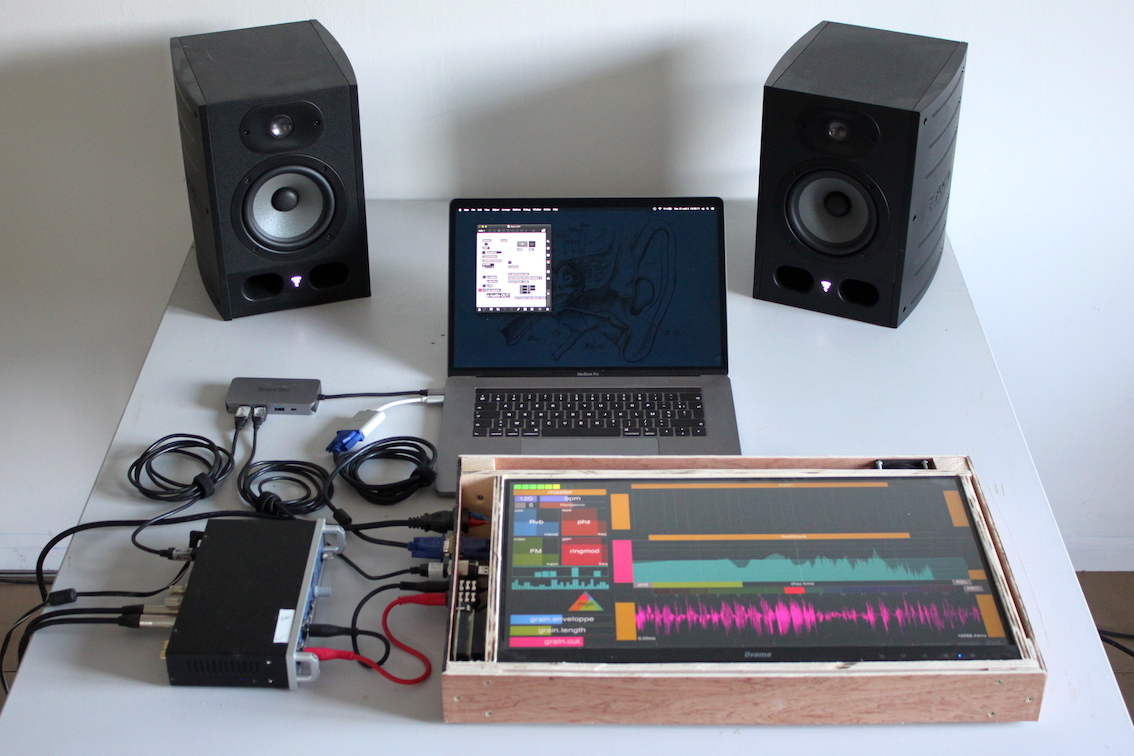
\includegraphics[width=\linewidth]{gfx/05_interfaces/Xypre_Overview_144dpi.jpg}
		\caption[Xypre: vue d'ensemble]{Xypre, vue d'ensemble: xypre, ordinateur avec Max, carte son, haut-parleurs}
		\label{fig:interface:xypre_unplugged}
	\end{minipage}
\end{figure}
%------------ Figure : filigramophone et xypre piezo -----------

%--------------------------------------------------------------
\section{Différentes faces de l'interface}

\subsection{Interface gestuelle ou interface sensible?}


\noindent Il est souvent question ``d'interface gestuelle'', voire de ``contrôleur gestuel'', lorsqu'on pense aux \glspl{IHM} utilisées pour l'interaction musicale. Comme nous l'avons vu au chapitre précédant, le geste y occupe une part importante, mais les interfaces de jeu ne se limitent pas nécessairement à la captation du geste : elle peuvent être sensibles à la température, la lumière\footnote{Voir par exemple les œuvres \textit{Light Thing} de Leaf Cutter John (\url{https://youtu.be/2jIlLHfSEfs}), ou encore \textit{Light Music} de Thierry de Mey}, la couleur, la géolocalisation\footnote{Voir en particulier les travaux d'Atau Tanaka \cite{tanaka_mobile_2004}, ou les instruments de Yann Seznec \url{https://www.impracticaldevices.com}}, aux signaux biologiques internes du corps\footnote{Voir notamment les travaux de Marco Donnarumma \cite{donnarumma_biophysical_2017}} et réagir de manière générale à différentes conditions environnementales.\\
\indent Par ailleurs, le geste possède un certain nombre de qualités qui ne sont pas forcément captées par l'interface, alors qu'elle sont effectivement vues et ressenties par le musicien et par le public, et contribuent ainsi à la performance, comme nous l'avons présenté au chapitre précédent.\\
\indent Enfin, le ``geste'' qui vient contrôler les processus sonores dans les \glspl{DMI} peut être de nature virtuelle, prendre la forme de motifs pré-enregistrés qui peuvent être issus de toute sorte de source de données interprétées en tant que flux temporels, tels que peut-être le cas dans la sonification de données ou l'utilisation de ``modèles intermédiaires''\footnote{La notion de ``modèle intermédiaire'' sera décrit plus en détail dans le chapitre \ref{ch:algorithms}}.\\
\indent Pour toutes ces raisons, il semblerait ainsi préférable de parler d'\textit{interface sensible}, plutôt que d'\textit{interface gestuelle} pour décrire les dispositifs d'interaction numériques pour la musique, leur caractéristique commune étant l'usage de capteurs (\textit{sensors}).
\indent Inversement, les haut-parleurs, les projections graphiques, les moteurs et actionneurs contrôlés algorithmiquement sont également \textit{à l'interface}, en ``sortie'' cette fois, entre le virtuel et le réel. Si de même, on considère plus souvent la partie ``captation'' que la partie ``diffusion'' lorsqu'on évoque les interfaces de jeu des \glspl{DMI}, il faut garder en vue que ces deux aspects s'entremêlent, non seulement dans la boucle de rétro-action qui se créé entre le musicien et l'instrument, mais également dans l'agencement concret des éléments matériels qui constituent le dispositif instrumental dans son ensemble, comme nous le verront dans ce chapitre.\\
\indent L'interface de jeu, en étant sensible à son environnement tout en rendant perceptible les artefacts générés par les algorithmes, vient incarner la potentialité virtuelle d'un \gls{DMI}.


%%%%%%%%%%%%%%%%%%%%%%%%%%%%%%%%%%%%%%%%%
\subsection{Un support pour \textit{musiquer}}

\noindent Les \glspl{DMI} sont des objets techniques dont l'interface est le support de diverses activités musicales, allant de la composition à la performance, en passant par la pédagogie. En tant qu'agencements éphémères en perpétuelle évolution\footnote{Cf. chapitre \ref{ch:ephemeral}}, leur interface est parfois le support de l'activité même de lutherie qui sert à les concevoir\footnote{L'exemple le plus manifeste de cette amalgame entre les fonctions d'instrument de performance, de composition et de lutherie est sans doute le \textit{live-coding}, dans lequel le clavier alphanumérique (ainsi que l'écran et les haut-parleurs) joue le rôle d'interface de jeu polyvalente pour ces différents contexte.}.

\noindent Les \glspl{DMI} intègrent souvent des matériaux sonores pré-composés, que le musicien peut déclencher et qui pourront tourner de manière autonome (paysages sonores, processus génératifs, drônes, etc.) et une part créée plus directement, qu'elle soit synthèse ou transformation de matériaux.\\
\indent Les différents accès de l'interface de jeu doivent ainsi permettrent d'articuler ces deux pôles, en permettant la gestion du temps à différentes échelles. En particulier, les écrans \textit{multitouch}, s'ils permettent de gérer aisément de multiples processus lents (qu'on pourra visualiser et ajuster à l'écran), ne permettent guère une réactivité ``percussive'', telle que le permet un pad \gls{MIDI} ou un capteur échantillonné à fréquence audio.\\
\indent La granularité du contrôle joue également un rôle important dans cette perspective. Entre une note \gls{MIDI} qui ne déclenche qu'un événement ponctuel, un contrôleur continu qui envoie des données chaque fois qu'il est modifié et un capteur échantillonné à fréquence audio qui envoit ses valeurs 44100 fois par seconde, les possibilités de contrôle seront différentes en terme de réactivité et de finesse de modulation. Il faut donc prévoir les capteurs adéquats pour les processus que l'on souhaite contrôler en aval. Comme le faisait remarquer Max Mathews: \iquote{Il faut penser aux systèmes dans leur globalité pour obtenir une quelque chose d'utilisable musicalement - on ne peut pas vraiment développer un capteur sans le mettre en perspective des programmes avec lesquels on va l'utiliser}\footnote{``One has to think of overall systems to get a musically useful thing — you can't really develop a sensor without relating it to the programs that you're going to use it with.'', Max Mathews, cité par Joel Chadabe dans \cite{chadabe_electric_1996}, p. 230}.\\
\indent Ceci n'est pas sans poser problème dans la perspective de modularité d'un \gls{DMI} que l'on aimerait pouvoir faire évoluer et adapter à différents contextes. Un compromis consiste à disposer d'une palette de capteurs différents afin de les agencer selon une ergonomie adaptée aux gestes qu'ils invitent, et d'adapter le logiciel, plus souple, à cette configuration. \todo{améliorer cette partie}

\subsection{Instruments acoustico-électronico-numériques}

\noindent Si on les considère sur le plan matériel, il faut encore noter que les \glspl{DMI}, s'ils se caractérisent par l'usage de la computation numérique, sont aussi nécessairement des instruments électroniques, électriques et acoustiques. Il portent par conséquent l'héritage et les contraintes propres à ces différentes dimensions.\\
\indent Dans le domaine virtuel du code informatique, ces dimensions sont (trop\footnote{Cf. commentaires en section \ref{ch:algorithms:digital-material}}) bien séparées : la mécanique et l'électricité y sont absentes, et les signaux acoustiques et de contrôle bien rangés dans des variables indépendantes qui n'interagissent que si on le leur demande explicitement. Dans le monde réel, au contraire, l'interférence est la règle --~pour le meilleur et pour le pire~-- et il devient nécessaire d'isoler les différents signaux si l'on ne veut pas avoir à gérer la complexité de leur interaction : mettre les haut-parleurs loin des microphones, isoler les câbles électriques pour ne pas capter la radio, rajouter des mousses pour ne pas entendre les bruits mécaniques d'une frappe sur un capteur, etc. L'interface de jeu est cette partie d'un \gls{DMI} qui doit communiquer avec le virtuel mais aussi composer avec le réel.

%-------------------------------------------------------------

\section{Facteurs de formes: héritages et transpositions}
\label{sec:interfaces:heritages}

\subsection{Héritage instrumental}

\noindent Les \glspl{DMI}, en partie libérés\footnote{cf. § \ref{sec:interfaces:part_acoustique}} des contraintes de facteur de forme liées à l'acoustique, présentent un agencement et une topologie liés à des questions d'ergonomie d'une part mais aussi d'héritages, instrumentaux ou non. L'héritage le plus évident est celui des techniques de jeu et du répertoire, qui prend une importance considérable dans le design des \glspl{DMI} inspirés d'instruments pré-existants, en particulier les instruments dits augmentés (cf. Annexes \ref{appendix:turchet} et \ref{appendix:mamou-mani}). Cet héritage est le plus manifeste dans les instruments destinés au commerce, en permettant un effet dilligence\footnote{notion définie par le médiologue Jacques Perriault, décrivant les protocoles mis en place pour l'adaptation d'une innovation en vue de son acceptation sociale (``Les premiers wagons avaient la forme des diligences.'')} entre instruments classiques et instruments nouveaux.\\

TODO : inclure une image de la HyVibe et/ou de l'hyper mandoline de Turchet.\\
Héritage des techniques de jeu et du répertoire : cf. interview Adrien MM et Lucas Turchet) 


\subsection{Héritage du corps}
\noindent L'ergonomie, pensée en dehors de l'organologie classique, nous amène à considérer directement le corps, et plus particulièrement les mains. Comme l'explique Serge de Laubier (cf. Annexe \ref{appendix:delaubier}) :\\
\iquote{(...) quand on fabrique un instrument il y a une contrainte, c'est le corps et donc forcément, il faut que les instruments, en tout cas ceux qui fonctionnent bien, soient quand même relativement bien adaptés au corps... relativement parce que, même les instruments acoustiques, les instrumentistes se détruisent pas mal mais quand même, malgré tout, il arrivent à les pratiquer pendant des années, plusieurs heures par jour, et en général ils tiennent... donc la contrainte du corps est importante et la première contrainte c'est celle des mains, avant la contrainte du corps... parce que c'est le plus agile je pense, le plus agile, rapide, réactif}\\

Un certain nombre d'instruments comme ``The Hands'' de Michel Waisvisz ou le Méta-Instrument de Serge De Laubier sont ainsi directement conçus à partir de l'ergonomie de la main, de la mécanique du corps.

\subsection{Héritage de l'objet}

\noindent L'instrument est également un objet de scénographie et c'est parfois sa fonction scénographique qui initie et oriente le développement de l'instrument. C'est par exemple le cas dans l'usage d'objets détournés, tels que ``The Sponge'' de Martin Marier \cite{marier_sponge_2010}, ou dans les installations de Patrick Saint-Denis qui \iquote{part de l'objet} et \iquote{poursuit l'idée des objets animés par le son} (cf. Annexe \ref{appendix:saint-denis}).\\

TODO : mettre une image de The Sponge et des accordéons de Patrick Saint Denis

%%%%%%%%%%%%%%%%%%%%%%%%%%%%%%%%%%%%%%%%%
\subsection{Héritage poétique}

\noindent Une autre forme d'héritage est celui de l'imaginaire, de la force d'évocation poétique des objets, qui dépasse le strict cadre fonctionnel de la relation instrumentale. Cet imaginaire polarise le jeu du musicien et l'écoute du public, \iquote{comme s'il y avait un arrière plan imaginaire de tout ce que ça draine d'histoire, de projections} (cf. Annexe \ref{appendix:dumeaux}). On retrouve la même fonction de détournement d'objets et d'association imaginaire dans ``l'Olitherpe'', instrument joué par Patricia Dallio, qui se présente comme un agencement de capteurs intégrés dans des objets de récupération. 

\begin{quotation}
	J'ai l'habitude de récupérer des objets qui me parlent. Je ne sais pas pourquoi il me parlent, mais ils me parlent. J'ai pu associer des mouvements aux formes des objets. (...) Le mouvement m'inspirait l'objet, ou l'objet était en corrélation avec le mouvement. C'est aussi une de mes habitudes de récupérer et de savoir ce que j'ai dans mes affaires et de pouvoir l'intégrer à quelque chose d'utile et de pratique qui n'est pas forcément son but d'origine.
\end{quotation}

\noindent Dans un documentaire\footnote{Documentaire ``L'Olitherpe et la teneur de l'air'' : \url{https://vimeo.com/224494409}}, Olivier Charlet qui s'occupe de la construction du dispositif (intégration des capteurs dans un habillage et une structure) évoque plusieurs pistes qui orientent l'intégration des capteurs : 
\vspace{-1em}
\begin{itemize}[noitemsep]
\item \textbf{l'usage qu'en fait la musicienne} dans son jeu, dont on peut imaginer qu'il conditionne l'endroit du dispositif où le nouveau capteur sera intégré; 
\item le \textbf{fonctionnement propre des capteurs} : par exemple un capteur de distance qui envoie un signal infra-rouge et reçoit sa réflection nécessitera un espace libre dans son champ de captation;
\item une \textbf{association morphologique} entre le mouvement de l'instrumentiste et la forme de l'objet;
\item des \textbf{associations imaginaires et poétiques} : le capteur infra-rouge évoque des yeux et c'est dans un vieux phare de vélo récupéré qu'il sera intégré, choisi pour ses qualités évocatoires (``J'ai l'habitude de récupérer des objets qui me parlent.'').
\end{itemize}

\noindent On peut voir dans la démarche artisanale et \gls{DIY} des lutheries numériques l`importance accordée à la charge affective des objets; les contrôleurs numériques (tels que les contrôleurs \gls{MIDI}) vendus dans le commerce sont en effet souvent issus d'une production industrielle et faits de matériaux plastiques qui à l'inverse du bois d'un violon, ne porte pas la trace organique des fibres du bois ou celle du geste artisanal imprimé par le luthier et se retrouve, d'une certaine manière, dépourvu d'histoire.

%%%%%%%%%%%%%%%%%%%%%%%%%%

\section{Matériaux}
\label{sec:interfaces:materials}

%-------------------------- Figure : table du luthier numérique ----------------------------------
\begin{figure}[!htbp]
	\captionsetup{format=plain}%
	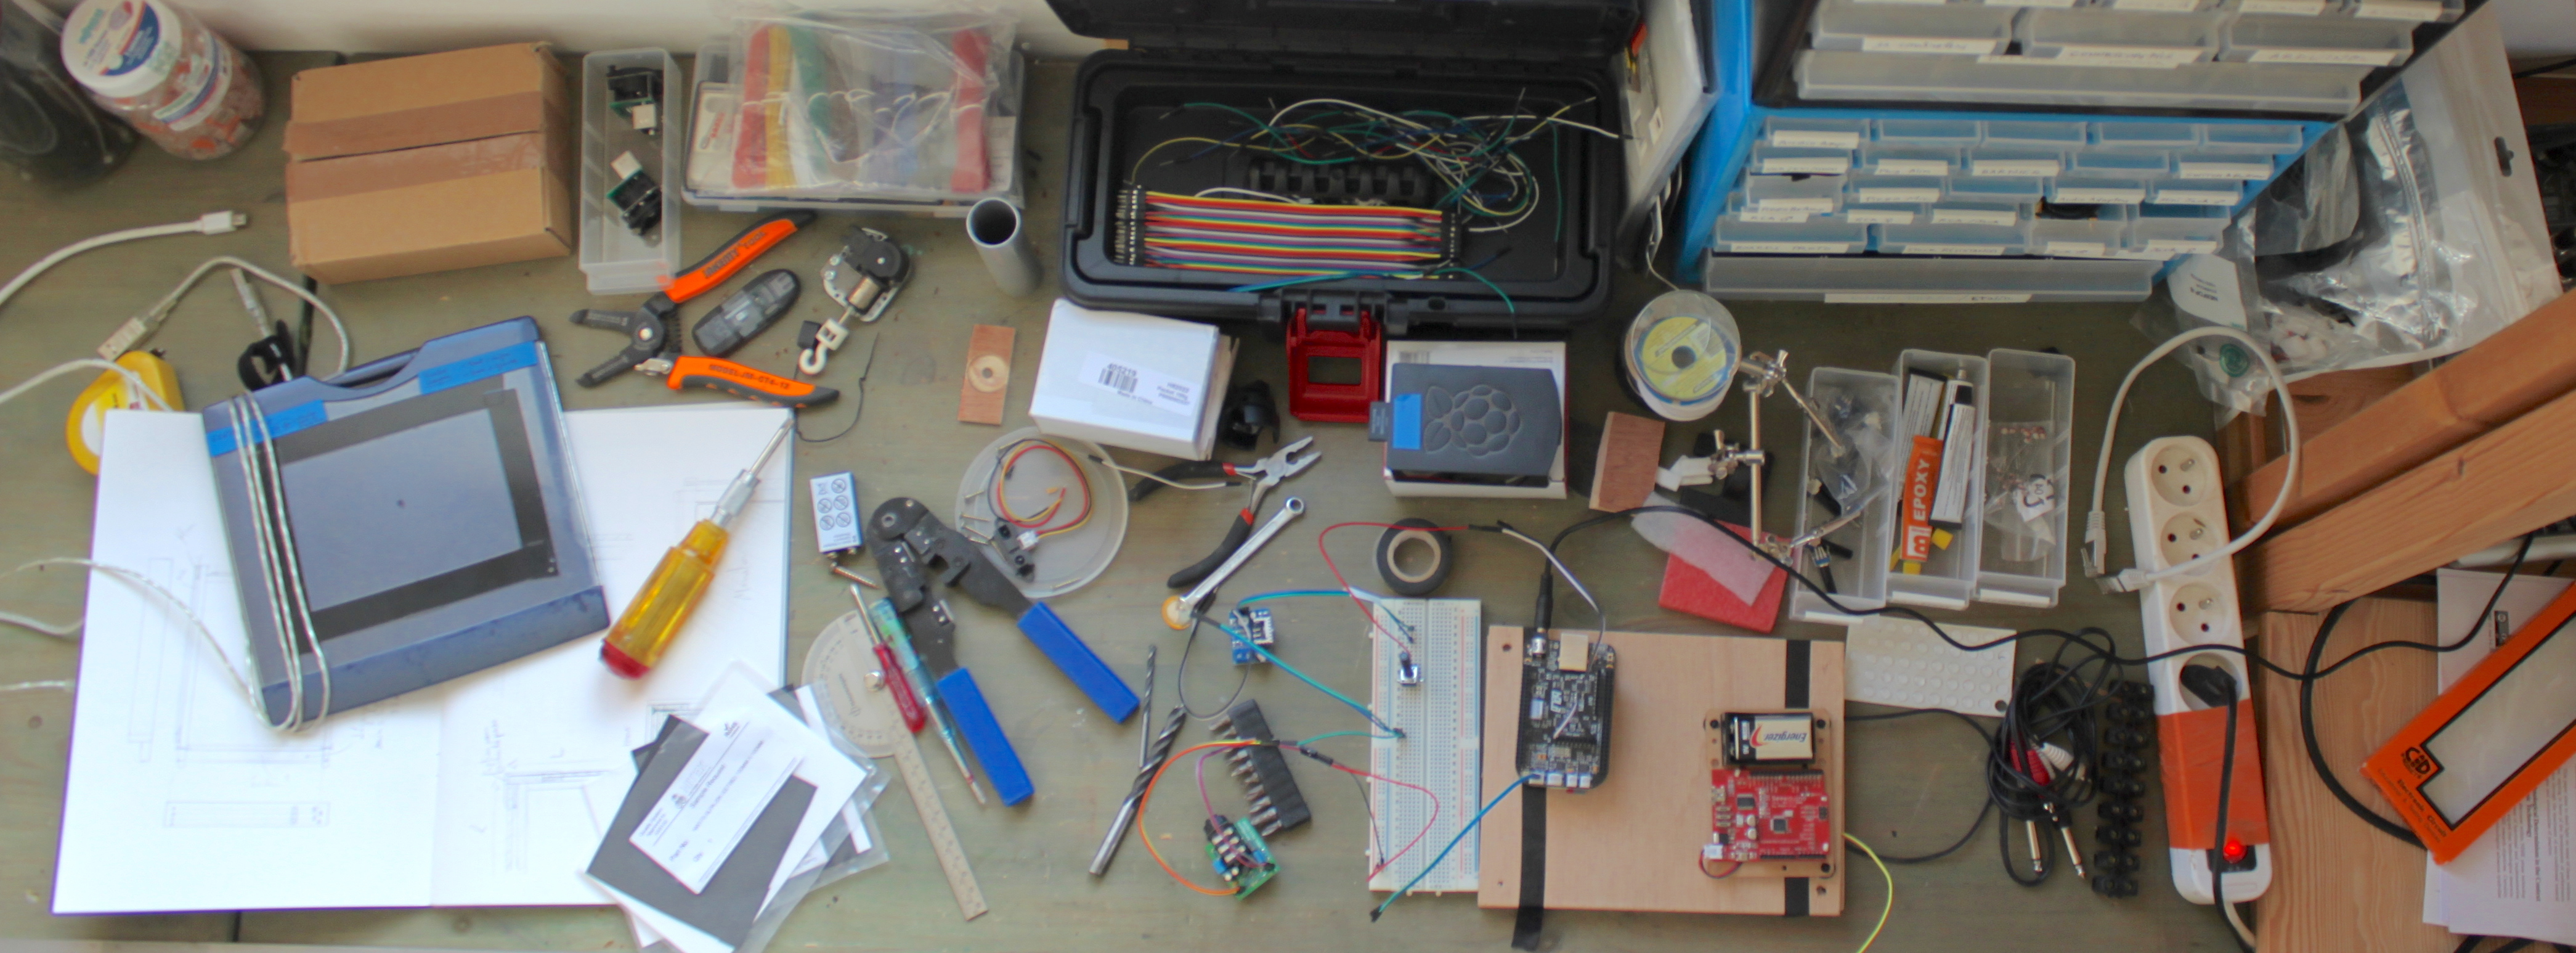
\includegraphics[width=\textwidth]{gfx/05_interfaces/lutherie-worktable.jpg}
	\caption[Matériaux sur la table d'un luthier numérique]{Matériaux sur la table d'un luthier numérique.}
	\label{fig:interface:table-luthier}
\end{figure}
%-------------------------- Figure : table du luthier numérique ----------------------------------

\noindent Cette section regroupe un ``fatras'' d'éléments matériels qui peuvent se retrouver sur la table de travail d'un luthier numérique. Il aurait été tentant de les séparer en une catégorie ``matériaux bruts'' d'une part et ``électronique'' d'autre part, mais ç'aurait été masquer l'interpénétration croissante de ces deux champs. D'une part, les matériaux ``bruts'' sont en fait rarement bruts au point d'être ``naturels'' (e.g. une plaque de contreplaqué ne pousse pas dans la nature), et d'autre part, l'intégration de l'électronique confère souvent un rôle à des matériaux qui ne le sont a priori pas électriques\footnote{Considérons par exemple le cas d'un chassis métallique, dont la fonction est avant tout structurelle, et qui est relié à la masse.}.\\
\indent Je présente ici une liste non-exhaustive de matériaux pouvant se retrouver sur la table de travail d'un luthier numérique, ainsi que le rôle qu'ils jouent dans la fabrication d'une interface de \gls{DMI}. Bien que ces catégories s'interpénètrent, ils sont envisagés selon trois perspectives : matériaux structurels, captation et computation, objets détournés.

\subsection{Matériaux structurels}

Les matériaux structurels définissent l'agencement physique du \gls{DMI}, non seulement la distribution spatiale de son affordance mais également la cohésion et les liaisons mécaniques entre les différents capteurs. En effet, on touche rarement les capteurs de manière directe : ils sont recouverts, enveloppés, intégrés dans un objet matériel plus ou moins complexe, possédant son propre état de surface, son propre jeu mécanique, en liaison avec le reste du dispositif.
Ils assurent la jonction autant que l'isolement des différent capteurs.

Usinage
=> propriétés acoustiques, mécanique (résistance, élasticité), électriques, électromagnétiques, transparence de	ces matériaux, état de surface (poreux, lisse), matériaux ``travaillables'' (e.g. collable,perçable, vissable)
=> disponibilité et forme sous laquelle ils sont vendus (e.g. plaques de bois, textile au mètre, etc.)

\vspace{-1em}
\begin{itemize}[noitemsep]
	\item \textbf{le bois}: Le contreplaqué est très souvent utilisé pour le prototypage rapide des \glspl{DMI}. Disponible en plaques de différentes épaisseurs, facilement découpable, perçable, collable et usinable par machine \gls{CNC}, il est un matériau très répandu dans la fabrication \gls{DIY} et les \glspl{makerspace}. Mais par ailleurs, le bois est historiquement le matériau phare de la lutherie acoustique. Il est par conséquent présent dans les instruments augmentés issus de lutheries acoustiques. Son importance historique l'ancre dans l'imaginaire collectif de l'instrument de musique. L'image d'Epinal de l'atelier du facteur d'instrument est remplie de copeaux et de ciseaux à bois et, de même que le public reconnait un dispositif électronique comme instrument de musique à partir du moment où l'on branche un clavier dessus\footnote{Cf. l'analyse de Trevor Pinch dans \cite{pinch_why_2001}}, le bois contribue à donner un sentiment d'instrumentalité à un dispositif numérique. Ainsi, bien que n'ayant aucun rôle fonctionnel, le bois massif est utilisé pour son caractère noble et évocateur sur certains instruments numériques high-tech, tels que le Linnstrument, le SoundPlane (todo : photos).
	\item \textbf{le métal} est couramment utilisé pour les chassis et les coques de revêtement des machines électriques et électronique. En dehors de ses propriétés de résistance mécanique, sa conductivité permet d'isoler les composants de faux contacts et de perturbations électromagnétiques et notamment d'éviter le ``bruit de masse'' qui peut survenir quand un équippement électrique tel qu'un \gls{DMI} n'est pas relié à la masse. Le métal possède également des propriétés de résonance acoustique qui en font un matériau intéressant pour la captation et la diffusion électro-acoustique, et utilisé par exemple dans le diffuseur ``Gong'' de l'onde Martenot.
	\item \textbf{le plastique} offre de grande facilités de thermoformage, moulage, collage, perçage, gravage, qui permettent d'obtenir toute sorte de forme et notamment de s'adapter à l'ergonomie du corps (e.g. la main du MI). Les propriétés de transparence du \gls{PMMA}\footnote{aussi connue sous le nom commercial Plexiglass} permettent de l'utiliser au dessus d'un écran. L'essor des imprimantes 3D depuis le début du \siecle{21}~siècle a également contribué à son utilisation pour le prototypage rapide dans un contexte autre qu'industriel, et de pratiques \gls{DIY} dans les \glspl{makerspace}. (todo : photo main MI4?)
	\item \textbf{le verre} a été utilisé en particulier pour le caractère cristallin de sa résonnance acoustique (e.g. Cristal Baschet, glass-harmonica). Plus difficile à travailler, ses proprétés de transparence, et de résonance (cf. projet résonance auto NIME 2019)
	\item \textbf{la mousse} est généralement utilisée pour ses propriété d'isolation phonique et vibratoire, mais également comme matériau tampon, pour augmenter la course des capteurs de pression (\gls{FSR}). Il existe de nombreuses sortes de mousses, offrant des nuances différentes d'enfoncement, de résiliance et affectant considérablement la sensation tactile sur ce type de capteurs.
	\item \textbf{le textile} a enfin été utilisé dans un certain nombre de \glspl{DMI} et de manière plus générale dans tout le champ d'interaction entre le domaine de la confection textile et de l'électronique, généralement désignée sous le terme de ``\textit{wearable electronics}''\footnote{Cf. la revue proposée dans \cite{stoppa_wearable_2014}}. La possibilité d'intégrer des fibres conductrices entrelacées dans le textile (``\textit{e-textile}'') a ainsi donné lieu à plusieurs développements de surfaces multitouch \cite{freed_application_2008, donneaud_designing_2017, wicaksono_fabrickeyboard:_2017} ou de vêtements munis de capteurs \cite{hayafuchi_musicglove_2008, serafin_controlling_2014, myllykoski_prototyping_2015}.
\end{itemize}

\noindent En dehors de ce matériaux relativement bruts qu'il s'agit d'assembler, les lutheries numériques opèrent aussi de manière ``sauvage'' en s'appropriant des objets déjà complexes et en les détournant à de fins musicales nouvelles, comme il a été présenté dans la section \ref{sec:interfaces:heritages}.

%%%%%%%%%%%%%%%%%%%%%%%%%%%%%%%%%%%%%%%%%%%%%%%%%%%%%%%%%

\subsection{Capteurs}

\noindent Une grande diversité de capteurs est disponible sur le marché, mesurant différentes grandeurs physiques : position, distance, pression, orientation, flux d'air, lumière, humidité, température, champ magnétique, présence, contact, etc. Leur utilisation spécifique dans le domaine des lutheries numériques a été l'objet de nombreuses études qualitatives et quantitatives, menées en particulier depuis ces deux dernière décennies par l'équipe de Marcello Wanderley à l'\gls{IDMIL}\footnote{Voir notamment : \cite{wanderley_choice_2000, hollinger_evaluation_2006, marshall_sensor_2009, vigliensoni_quantitative_2012, medeiros_comprehensive_2014} ainsi que le site \url{https://sensorwiki.org} qui rassemble un grand nombre d'informations techniques utiles sur les capteurs et les interfaces}.

Les capteurs ne sont que des ``portes d'entrées'' de la partie algorithmique d'un \gls{DMI}. 

Outre le type de grandeur mesurée, les capteurs se distinguent entre ceux qui permettent une mesure stable (e.g. position d'un potentiomètre), ou dynamique, c'est à dire qui revient à une valeur de repos quand on le relâche (capteur de distance, de pression)

Comme dit précédemment, les capteurs sont généralement intégrés dans un enrobage matériel, voire un système mécanique complexe, qui peut pour un même capteur donner lieu à des interactions tout à fait différentes. 

On peut regrouper les capteurs dans deux grandes familles
Capteurs ``bruts'' et capteur ``intelligents''
Pads MIDI => peuvent être implémentés via interrupteurs, piezzo, FSR...
Multitouch = différentes technologies de détections (capacitives, infra-rouge, etc.) pour renvoyer la position des doigts.

\indent Un certain nombre d'études ont par ailleurs proposé une analyse de l'adéquation entre capteurs et fonctions musicale (e.g. \cite{vertegaal_towards_1996, goudeseune_interpolated_2002}), en mettant les aspects statique, dynamique, absolue ou relatif des valeurs transmises par les capteurs en regard de ces mêmes aspects appliqués à des grandeurs liées à la musique (en particulier le pitch), dans l'optique d'évaluer qualitativement l'adéquation entre le choix des capteurs et le type de contrôle musical\footnote{Cette perspective reflète de manière plus générale une tendance de l'époque à vouloir répliquer le modèle instrumental classique ou la relation entre le geste et le résultat sonore est très directe. La remarque en fin d'article \iquote{(...) a good causal mapping can ensure that tension is properly translated to the audible result.} en est révélatrice. Voir également la position de Claude Cadoz en ce sens au chapitre \ref{ch:gesture}}. Bien qu'instructives et utiles dans la perspective d'une relation de mimétisme univoque entre le mouvement gestuel et le mouvement d'un paramètre sonore, ces études mettent cependant de côté un aspect important des \glspl{DMI}, à savoir la possibilité sans pareil des ordinateurs à traiter le signal et transformer le continu en discret, l'absolu en relatif, le statique en dynamique, et inversement, et plus encore, si l'on sort de ce cadre relationnel univoque entre un capteur et un paramètre.\\
%-------------------------- Figure : Vertegaal-transducer-function ----------------------------------
\begin{figure}[!htbp]
	\captionsetup{format=plain}%
	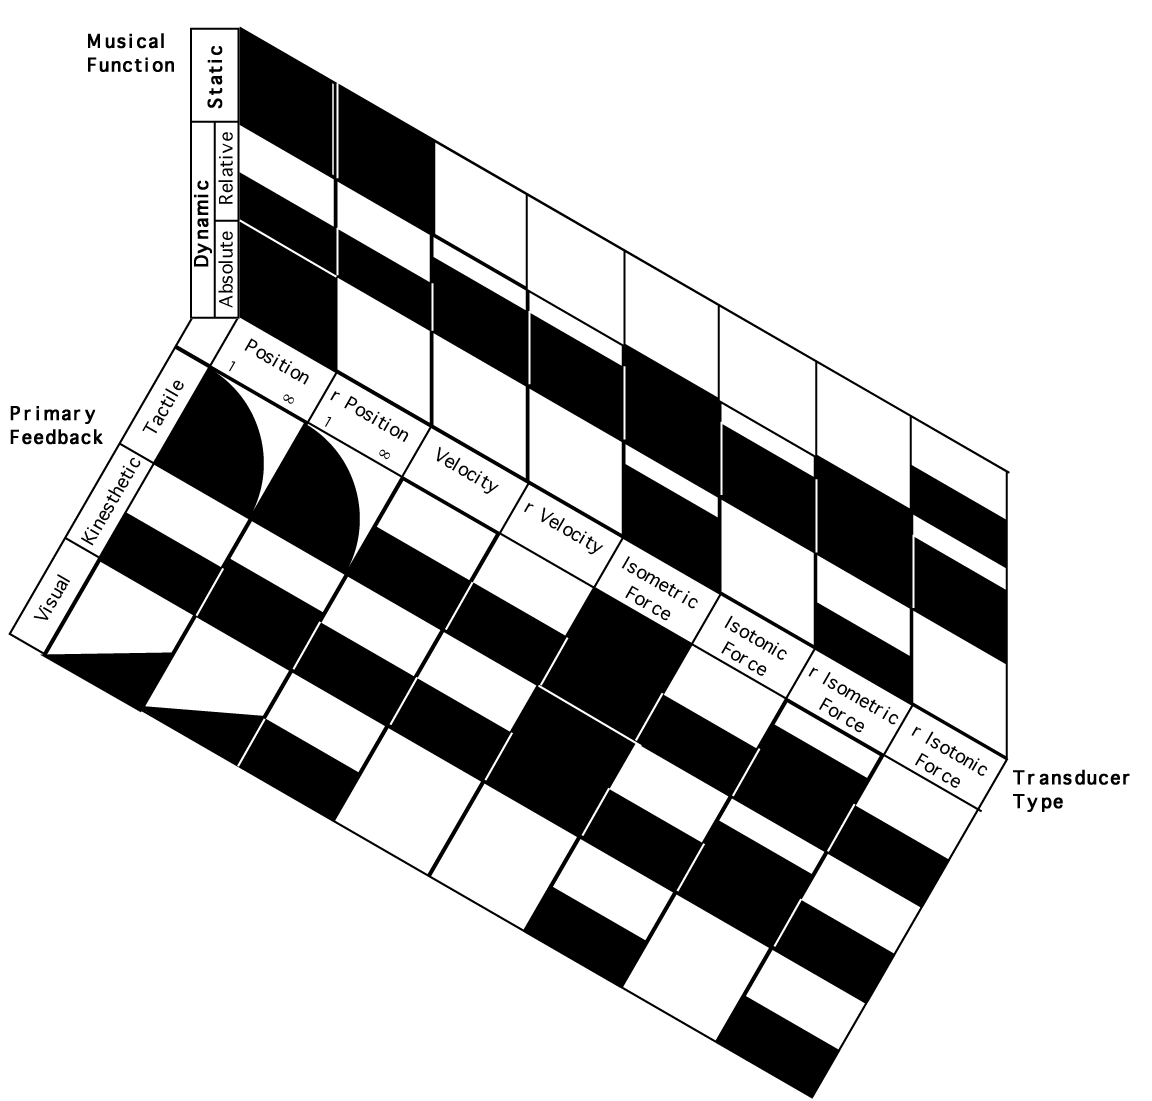
\includegraphics[width=\textwidth]{gfx/05_interfaces/vertegaal-musical-function.png}
	\caption[Adéquation entre fonction musicale, transducteur et retour primaire]{Adéquation entre fonction musicale, transducteur et retour primaire, selon \cite{vertegaal_towards_1996}.}
	\label{fig:interface:vertegaal-transducer-function}
\end{figure}
%-------------------------- Figure : Vertegaal-transducer-function ----------------------------------
\indent Ainsi d'après l'étude de Vertegaal (cf. figure \ref{fig:interface:vertegaal-transducer-function}), un potentiomètre linéaire serait très adapté à la sélection d'une valeur absolue de hauteur, tandis qu'un capteur de pression isotonique tel qu'un \gls{FSR} serait plus adapté à sa modulation. Ce modèle ``subjectif'' (selon les termes des auteurs\footnote{Cf. \cite{ungvary_cognition_1999}}) de Vertegaal et Ungvary a été ``confirmé'' expérimentalement par une étude récente \footnote{Cf. \cite{malloch_design_2019}}, mais dans un contexte de laboratoire. Il est ici intéressant de remarquer qu'un clavier de synthétiseur implémente quasiment l'exact opposé, en permettant de sélectionner des hauteurs absolues par un ensemble de capteurs de pression et de vélocité sous les touches tandis qu'un potentiomètre rotatif --~mais présenté latéralement, ce qui rend sa course longitudinale plutôt que radiale~--, le ``\textit{pitch-bend wheel}'' permet leur modulation relative. La différence par rapport au modèle thérorique d'Ungvary et Vertegaal tient au fait que le mapping n'y est pas \textit{one-to-one} en ce qui concerne la hauteur, que le potentiomètre du \textit{pitch-bend-wheel} est muni d'un ressort de rappel, et que ces deux capteurs contrôlent la hauteur de manière conjointe.\\
%-------------------------- Figure : table du luthier numérique ----------------------------------
\begin{figure}[!htbp]
	\captionsetup{format=plain}%
	\includegraphics[width=\textwidth]{gfx/05_interfaces/clavier-Martenot-MIDI.png}
	\caption[Agencement des capteurs et fonction musicale]{Un exemple de l'influence de l'agencement des capteurs sur leur usage musicale: à gauche l'Onde Martenet: slider linéaire pour le contrôle de hauteur (avec la bague) et capteur de pression pour la modulation (d'intensité). A droite, un clavier MIDI : multiples capteurs de pression pour la sélection de la hauteur absolue et potentiomètre pseudo-linéaire pour la modulation (pitch-bend).}
	\label{fig:interface:martenot-clavier}
\end{figure}
%-------------------------- Figure : table du luthier numérique ----------------------------------
\indent On voit donc que l'usage, la taille, l'agencement des capteurs et le traitement de ses données contribuent pour autant, sinon davantage, à définir les relations entre capteurs et paramètres musicaux, que la nature de la variation du capteur lui-même. Le fait qu'un paramètre musical ne soit pas ``facilement'' modulable avec un certain type de capteur ne présage donc pas de l'inadéquation de ce capteur pour le contrôle du paramètre en question. Tout au contraire, cela peut faire partie de la \textit{raison d'être} de l'instrument, dont la pratique peut s'apparenter davantage à celle du domptage d'un animal sauvage que celle de l'utilisation d'une machine docile\footnote{On pense par exemple au Theremin, sur lequel le contrôle de la hauteur par la distance de la main à l'antenne est très instable et difficile, et dont la maitrise est probablement un des intérêt de sa pratique. Quant au violon, il n'aurait tout simplement jamais vu le jour.}

Ce décalage entre l'évalutation des capteurs et leur usage réel provient \\


Question de latence : ``action-sound latency'' de A. McPherson

\subsubsection{Capteurs intelligents}

Fusion de capteurs, prétraitement

\noindent Cetains capteurs renvoient des données de plus haut niveau que la donnée brute, en la traitant au préalable localement au niveau du capteur lui-même. Par exemple, l'image renvoyée par une caméra est un signal multiplexé contenant les données de plusieurs millions d'éléments photosensibles intégrés dans un composant miniature. 
De même, les points de contact renvoyés par un écran multitouch sont issus d'un pré-traitement de la matrice de capteurs capacitifs ou photo-sensibles répartis sur une surface sensible.

\indent L'intelligence embarquée dans les capteurs est amenée à se développer, à mesure que progresse le traitement d'image et en particulier les algorithmes d'apprentissage par \gls{IA}, qui permettent d'extraire des contenus sémantiques, tels que la reconnaissance de motifs (objets, visages, mélodie, etc.).

\indent Cette évolution pose deux questions : 

L'extraction de données de plus haut niveau pose un problème général du modèle qu'on impose sur les données brutes (le dessein).


	Capteurs intelligents (IHM)
	cf \ref{appendix:delaubier}
	e.g. leap motion, multitouch overlays

\subsection{Interface d'aquisition}
	- ouverts et programmables
		- arduino, bela, teensy, etc.

\subsection{Ordinateurs et DSP}
\noindent L'arrivée concomittente de l'ordinateur personnel (PC), de la synthèse audio temps-réel et du protocole \gls{MIDI} dans les années 1980 a donné lieu à des dispositifs instrumentaux généralement constitués d'une interface de jeu d'une part et d'un \gls{DSP}, souvent un ordinateur, pour la synthèse d'autre part.

Depuis le début du \siecle{21}~siècle, de nombreux micro-controleurs, nano-ordinateurs ont vu le jour, permettant une ré-intégration de l'électronique numérique dans le corps de l'interface de jeu.
- raspberry pi, laptops, samplers and synths, smartphones


\subsubsection{Haut-parleurs et transducteurs tactiles}

\subsubsection{Actionneurs}
retour d'effort, moteurs de jeu acoustique (e.g. F. Collautti, robot musiciens), 

\subsection{La video}
projection, interface écran, cf. ch rep-viz

\noident Enfin, la description des dispositifs instrumentaux numériques ne serait pas complète sans mentionner les écran, les projecteurs, les actionneurs, les servo-moteurs, les lumières et tous les autres composants électiques contrôlés numériquement par le \gls{DMI}.


\section{La part acoustique de l'interface des DMIs}
\label{sec:interfaces:part_acoustique}

\noindent Il faut ici rappeler que les \glspl{DMI}, s'ils se caractérisent par l'usage de la computation numérique, sont aussi nécessairement des instruments électroniques, électriques et acoustiques. Il portent l'héritage et les contraintes propres à ces différents médias. Mais le phénomène acoustique, omnidirectionnel et tri-dimensionnel dans le monde physique, est réduit dans l'électronique numérique à un signal mono-dimensionnel\footnote{Nicolas Collins, dressant une liste de traits distinctifs entre hardware et software dans \cite{collins_semiconducting_2013} notait: ``Traditional acoustic instruments are three-dimensional objects, radiating sound in every direction, filling the volume of architectural space like syrup spreading over a waffle. Electronic circuits are much flatter, essentially two-dimensional. Software is inherently linear, every program is a one-dimensional string of code.''} et mono-directionnel\footnote{Au niveau logiciel, des blocs bi-directionnels de plus haut niveau peuvent cependant être crées, comme par exemple dans la librairie de modèles physiques pour \gls{FAUST}, cf. \cite{berdahl_introduction_2012} et \cite{michon_faust_2018}.}, introduisant une distinction entre les ``entrées'' d'une part et les ``sorties'' d'autre part. La dimension acoustique des \glspl{DMI} s'intègre donc dans un circuit ouvert ou fermé avec le système de computation via des transducteurs acoustiques --~microphones en entrée, ou haut-parleurs en sortie.\\
% \indent Par ailleurs, la vibration acoustique peut-être ressentie de manière auditive, quand sa transmission est aérienne, ou tactile lorsqu'elle est solidienne. Ces deux types de vibrations correspondent généralement à deux technologies de transducteurs différentes.
\indent Paradoxalement, si le résultat acoustique d'un instrument est \textit{in fine} ce qui nous intéresse le plus, la part acoustique de l'instrument numérique est aussi sa part maudite. Maudite au sens que lui donne George Bataille\footnote{La part maudite est la part d'énergie excédantaire, dissipée et gaspillée dans un luxe inutile.} d'une part dépensée et perdue dans la réduction par le microphone de la richesse du phénomène acoustique à un simple signal mono-dimensionnel autant que par le filtrage par les matériaux diffuseurs du signal audio qu'on leur envoit. Maudite également en raison du couplage épineux entre acoustique physique et audio numérique. Les phénomènes de résonnance et de rétro-action qui se produisent dans l'instrument acoustique et qui sont également exploités dans les instruments électriques analogiques (e.g. le feedback entre une guitare électrique et un amplificateur), posent un certain nombre de problèmes lorsqu'on introduit un élément de computation numérique dans un tel système\footnote{Une des raisons à ce problème est l'instabilité consubstantielle aux systèmes bouclés discrets et non-linéaires, mais également, de manière plus générale, la transition entre le domaine continu de l'acoustique et le domaine symbolique de l'informatique implique une analyse du son qui nécessite une modélisation des phénomènes perceptifs, tels que la hauteur, le rythme, etc. utilisés pour le contrôle}.\\
\extra{nombreux synthétiseurs analogiques ont été mis sur le marché, qui articulent cette part d'électronique analogique (pour les filtres et la synthèse) et numérique (pour le  contrôle), afin de pouvoir bénéficier des avantages des deux domaines.}

\subsection{Captation : microphones et transducteurs piezo}

\noindent La captation en direct de son acoustique dans un instrument électronique est une pratique très courante chez les musiciens électroacoustiques, qui permet des séquences de jeu en prise directe avec des sons concrets, amplifiés, enregistrés, transformés par l'instrument (ou non). En particulier, l'usage de microphones, notamment de transducteurs piezo dits ``microphone de contact'', vient redonner une composante acoustique au corps physique de l'agencement instrumental (et du musicien s'il utilise directement sa voix et son corps), cette composante acoustique ``naturelle'' étant sinon généralement couverte par la puissance du son amplifié. L'intérêt principal réside dans la richesse du signal capté, comme le note Miller Puckette\footnote{``(...) sliding a brush over a drum trigger isn’t likely to produce  anything  useful,  whereas  doing  the  same  thingon an instrument that operates directly on the audio signal from the contact microphone (as we do here) has the possibility to create a wide range of useful musical sounds.'' \cite{puckette_infuriating_2011}.} : \iquote{(...) il y a peu chance que le frottement de balais sur un pad de batterie produise quoi que ce soit d'intéressant, alors que faire la même chose sur un instrument qui fonctionne directement avec le signal audio du microphone de contact (comme nous le faisons ici) offre la possibilité de créer une large gamme de sons musicaux utiles.} L'usage d'algorithmes d'analyse en temps-réel permet, au-delà d'effets déjà existants dans le domaine électroacoustique, d'utiliser les caractéristiques du son comme paramètre de contrôle. Une telle approche a été utilisé notamment dans \cite{schwarz_rich_2014} et l'interface Mogees\footnote{\url{https://www.mogees.co.uk}, voir également l'Annexe \ref{appendix:zamborlin}} est principalement basée sur ce principe. 


\subsection{Diffusion : haut-parleurs et transducteurs tactiles}

\noindent Dans le cas le plus trivial, l'acoustique des \glspl{DMI} se limite à la membrane du haut-parleur qui transforme \textit{in fine} le signal audio-numérique en son acoustique\footnote{Le choix des haut-parleurs peut jouer un rôle primordial, comme c'est le cas dans la musique acousmatique diffusée sur orchestre de haut-parleur ou ``acousmonium''. Voir en particulier \cite{mooney_sound_2006}}. A la différence des instruments acoustiques, la diffusion et la projection du son est souvent séparée de l'interface gestuelle et, bien souvent, distante du musicien quand elle est ``spatialisée''. La spatialisation du son a en effet joué un rôle essentiel dans la motivation des concerts électroacoustiques ``live'', à une époque où l'arrivée du \gls{CD} est vendue comme la possibilité d'une écoute de salon ``haute-définition'' équivalente à l'expérience du concert\footnote{Comme en témoignent les publicités de l'époque, par exemple celle de Phillips mettant en scène un public les yeux bandés incapables de faire la différence entre le concert et l'écoute d'un \gls{CD}: \url{https://youtu.be/jtNyWmD3EQ4}}, comme le raconte Serge de Laubier en parlant des origines du PSO\footnote{``Processeur Spatial Octophonique'', système de spatialisation inventé par De Laubier en 1986.} et du Méta-Instrument (cf. annexe \ref{appendix:delaubier}) dans les années 1980 : \iquote{Si on entend mieux chez soi, c'est pas la peine de faire des concerts, donc il faut qu'au concert, il y ait une expérience unique qui vaille le coup de se déplacer, d'où réfléchir à un système de spatialisation.}\\
\indent L'essor progressif des transducteurs tactiles à large bande audio depuis la dernière décennie a cependant entrainé l'intégration de haut-parleurs dans le corps de l'instrument, en particulier dans les instruments augmentés tels que la Smart Guitar de HyVibe\footnote{\url{https://www.hyvibe.audio}}. Ce retour acoustique présente plusieurs intérêts :
\vspace{-1em}
\begin{itemize}[noitemsep]
	\item \textbf{offrir au musicien un retour vibratoire} (et/ou auditif), qui lui permet de mieux ressentir le résultat sonore et pouvoir plus facilement identifier sa contribution personnelle dans le cas de musique d'ensemble\footnote{Voir notamment };
	\item \textbf{faciliter l'identification et la localisation} auditive des instruments et accroître la lisibilité des relations geste/son pour le public;
	\item \textbf{bénéficier des propriétés acoustiques des matériaux} structurels de l'instrument, notamment leur rayonnement, beaucoup plus singulier que celui des haut-parleurs (dont la conception est généralement orientée vers un rayonnement homogène et une bande-passante plate);
	\item \textbf{introduire du feedback} dans le corps de l'instrument en recaptant cette vibration. Traité avec une latence suffisamment faible, cette possibilité laisse la possibilité de transformer dynamiquement les propriétés acoustiques des matériaux, comme le fait par exemple le système HyVibe\footnote{\url{https://hyvibe.audio}};
	\item \textbf{communiquer des informations} à l'instrumentiste via un retour vibratoire, tel que le frettage virtuel (cf. section TODO), ou des informations sémiotiques de plus haut-niveau\footnote{Voir en particulier le travail de Gabriela Patiño-Lakatos et al. \cite{patino-lakatos_paradigmes_2019} sur la communication intersubjective d'information par voie vibrotactile.}.
\end{itemize}



%-------------------------- Figure : PQlabs overlay ----------------------------------
\begin{figure}[!htbp]
	\captionsetup{format=plain}%
	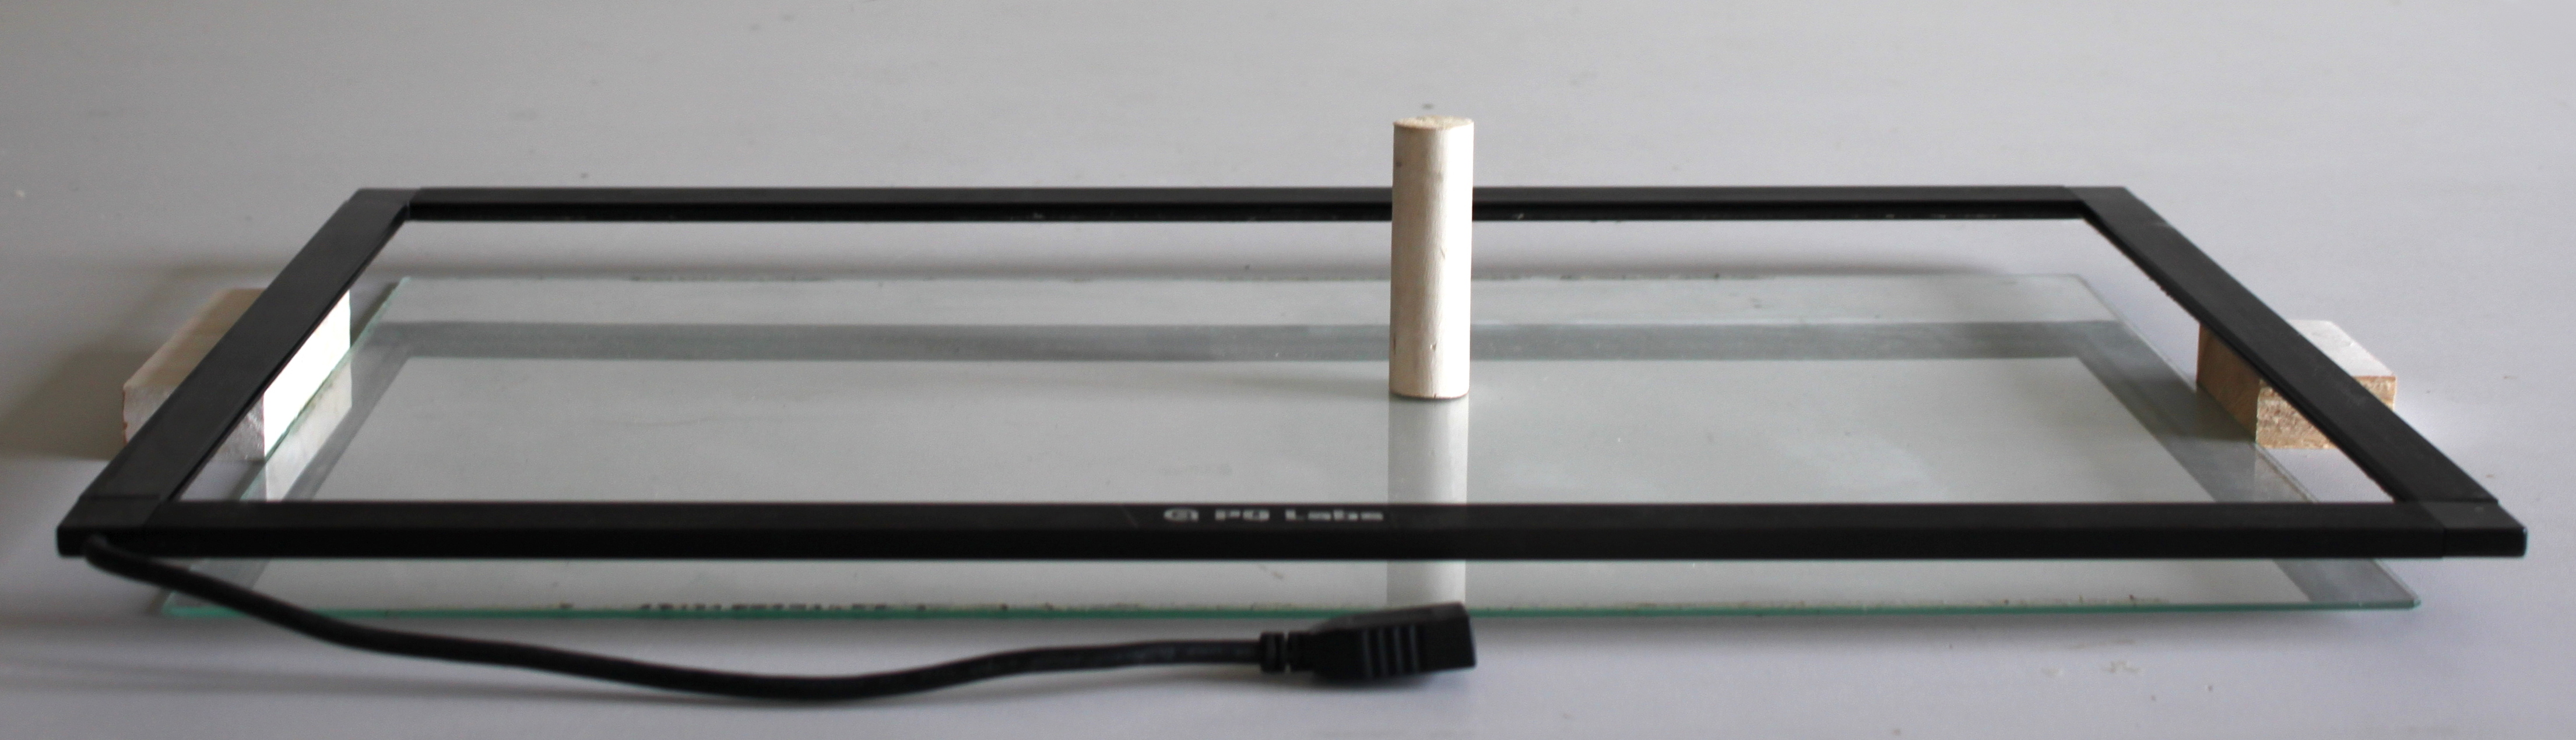
\includegraphics[width=\textwidth]{gfx/05_interfaces/PQlabs-G4overlay.jpg}
	\caption[Cadre multitouch à technologie infra-rouge]{Cadre multitouch à technologie infra-rouge (PQ-Labs). La surface de contact en verre est détachable et la captation d'objets quelconques est possible.}
	\label{fig:interface:PQlabs-G4overlay}
\end{figure}
%-------------------------- Figure : PQlabs overlay ----------------------------------



%%%%%%%%%%%%%%%%%%%%%%%%%%%%%%%%%%%%%%%%%
\section{Ergonomie, ergodynamisme}

%------------------------------------------------------------
\subsection{Ergodynamisme}

cf. définition de Thor Magnusson
agencement de l’interface, représentation visuelle, repères tactile, frettage


%------------------------------------------------------------
\subsection{Proprioception}

\noindent La proprioception désigne la perception de la position des différentes parties du corps dans l'espace, recouvrant le sens du mouvement (\textit{kinesthésie}) et le sens de la posture (\textit{statesthésie}). Dans le cas des \glspl{DMI}, cette proprioception est double : il s'agit à la fois d'intégrer la topologie réelle de l'instrument (disposition des capteurs, espace du mouvement autour de ceux-ci, course sensible et courbes de réponse...) mais également la topologie virtuelle des algorithmes manipulés. En ce qui concerne la topologie réelle de l'instrument, un aller-retour s'opère entre des gestes impliqués par le positionnement des capteurs et des gestes trouvés durant le jeu avec l'instrument.\\
\indent Ainsi, le positionnement des capteurs dans Xypre v2 a été revu en fonction de gestes qui venaient naturellement lors du jeu avec le filigramophone. Par exemple, le geste de percussion sur le côté du chassis venait naturellement dans la course du bras pivotant autour de l'articulation de l'épaule, alors qu'aucun capteur n'avait été positionné là. C'est par ailleurs un geste de percussion qu'on retrouve dans des instruments de percussion comme le Mridang indien, et que l'auteur ayant pratiqué le tabla trouvait relativement aisé.

\iquote{Though there is a huge range of performer decision, history, and knowledge that will determine their exact method of playing (as established by Jorda [12]), the physical design of the DMI impacts this gesture repertoire by presenting certain affordances.} \cite{bin_hands_2017}

Affordance

\subsection{Le poids du hardware}

\noindent Le hardware, comme son nom l'indique, est solide, matériel, ``dur''. Sa matérialité, son poids affecte sa transportabilité et constitue un facteur contraignant pour le musicien. Sa dématérialisation dans des alternative logicielles —\textit{soft}, plus douces et légères— permet ou non d'intégrer dans les limites acceptables pour leur transport des fonctionnalités offertes par les équipements \textit{hard}.
En particulier, la virtualisation des outils traditionnellement utilisés par les ingénieurs du son (table de mixage, équaliseurs, compresseurs et autres effets) permet leur intégration dans l'instrument lui-même.

(Cf. interview Mamou-Mani.)
Ainsi, Serge de Laubier qui utilisait une table de mixage Yamaha O2R (31kg) motorisée et contrôlée directement depuis son Méta-Instrument, ainsi qu'un échantilloneur EMU (4,5kg) a progressivement conçu des émulation logicielles de ces équipements pour alléger le transport. Par ailleurs, les émulations logicielles permettent de réaliser d'autres fonctions qui n'étaient pas présentes dans les modèles originaux.


\subsection{Portabilité et manipulation de l'interface}

Les instruments peuvent prendre différentes formes, plus ou moins grandes, qui définissent à la fois leur portabilité ainsi que la posture du musicien envers son instrument.
\vspace{-1em}
\begin{itemize}[noitemsep]
	\item interfaces portables, centrée sur le corps (e.g. exosquelette du MI3, Myo Atau Tanaka). L'instrument est \textit{porté} (un peu comme un habit) et les mouvements du corps sont directement, et en permanence captés par l'instrument.
	\item interfaces objets, topologie objet, qu'on peut prendre, secouer, etc. (e.g. ``The Sponge'' de Martin Marier) L'instrument est \textit{tenu} ou \textit{posé} (un peu comme un ustensile) avec les mains et manipulé ainsi.
	\item interfaces ``sur table'' objet qu'on ne peut pas déplacer mais autour duquel on peut tourner (e.g. claviers, pad, machine intona rumori de Bernier/Messier ...)
	\item interfaces immersives : installation, vidéo, danse (e.g.) (e.g. ``Machine variation'' de Bernier/Messier)
\end{itemize}

A noter que ces catégories ne sont pas étanches; par exemple, une guitare peut être portée, à l'aide d'une sangle, ou posée sur le genou et jouée à plat. 

\subsection{Intégration et temps de montage}

Est-ce que l'instrument est plug'n'play ou va-t-il va falloir connecter ses différents éléments ? Connections : 
\vspace{-1em}
\begin{itemize}[noitemsep]
	\item entre les capteurs et l'interface de digitalisation (arduino, carte son, etc.)
	\item entre le convertisseur analogique/numérique et l'ordinateur
	\item entre l'ordinateur et la carte son
	\item entre la carte son et les haut-parleurs
\end{itemize}

Les deux premières étapes sont absentes dans le cas du live-coding.

\noindent L'agencement des différents modules qui composent un \gls{DMI} entraine une facilité variable de transportabilité et un temps de démontage/remontage de l'instrument avant qu'il soit possible d'en jouer. Par ailleurs, les instruments électrifiés nécessitent généralement d'être branchés (sauf s'ils fonctionnent entièrement sur batterie). Ces branchement prennent du temps et nécessitent d'avoir des alimentations en courant à proximité. Pour les outils numériques se rajoute à cela le ``temps de lancement'', c'est-à-dire généralement le temps de démarrer l'ordinateur, de lancer le(s) logiciel(s) nécessaire(s), d'ouvrir le patch ou le script adéquat, et éventuellement de l'initialiser avec la bonne configuration.\\
\indent L'idéal d'un instrument numérique est souvent qualifié de ``\textit{plug'n play}'', mais rares sont les cas d'instruments qui s'affranchissent du ``\textit{plug}'' qui peut s'avérer long. Il est important de prendre en compte cette durée dans le design d'un \gls{DMI}, car tout le temps passé sur la partie de montage technique est pris au détriment du temps de jeu\footnote{...comme le font remarquer Nicolas Bernier (annexe \ref{appendix:bernier}), François Dumeaux (annexe \ref{appendix:dumeaux}) et Bruno Zamborlin (annexe \ref{appendix:zamborlin}) dans les entretiens)}. Notons toutefois que les \glspl{DMI} ne nécessitent généralement pas de temps d'accordage, et ne sont pas généralement pas sujets aux conditions de température et d'hygrométrie qui nécessite le ré-accordage des instruments acoustique et le temps de chauffe, particulièrement important pour les cuivres.

\subsection{Se repérer dans l'interface}

\subsubsection{Repères visuels}
Cf. section représentation visuelle

\subsection{Se repérer au toucher}
\indent Un grand défaut des interfaces graphiques ``tactiles'' est que leur surface est généralement dépourvue de repère tactile: aucune aspérité ne vient guider la main pour qu'elle trouve ses repères et son chemin sans l'aide de la vue. Différentes stratégies peuvent venir partiellement compenser cette lacune. Leur application dépend à la fois de la technologie de captation du \textit{multitouch}, ainsi que du type de repère, statique ou dynamique, que l'on souhaite.

\subsubsection{Repères statiques}
todo : parler des partitions tangibles d'Enrique Tomas

\noindent L'ajout de repères statiques ad-hoc et interchageables aide le toucher à sentir une position de repère sur l'écran tacile, ou encore les contours d'une zone d'interaction. Les interfaces ``Joué''\footnote{\url{https://www.play-joue.com}} ou ``Sensel Morph''\footnote{\url{https://sensel.com}} commercialisent différents revêtements (\textit{overlays}) pour leur surface \textit{multitouch}. Ces surfaces ne sont toutefois pas pourvue d'un écran graphique, ce qui évacue le problème de la transparence de ces repères.\\
Une solution bon marché consiste à utiliser de la bande adhésive (cf. figure \ref{fig:interface:filigramophone-adhesif}
). Un intermédiaire plus fin entre l'éphémère bande adhésive et une solution fixe consiste à utiliser une plaque de \gls{PMMA} (cf. figure \ref{fig:interface:filigramophone-plexigravure}) intermédiaire entre le doigt et la surface tactile, qui permet de graver des motifs potentiellement plus complexes. Cette dernière option n'est toutefois pas toujours réalisable sur les écrans à technologie capacitive, qui nécessite parfois que le doigt soit directement en contact avec l'écran.\\

%------------ Figure : repères statique -----------
\begin{figure}[!htbp]
	\captionsetup{format=plain}%
	\centering
	\begin{minipage}[t]{0.48\textwidth}
		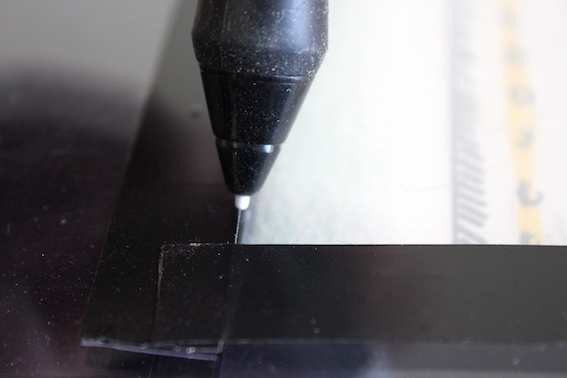
\includegraphics[width=\linewidth]{gfx/05_interfaces/filigramophone-adhesif_72dpi.jpg}
		\caption{Bande adhésive permettant de sentir le contour de la zone sensible de la tablette}
		\label{fig:interface:filigramophone-adhesif}
	\end{minipage}
	\hspace{.02\linewidth}
	\begin{minipage}[t]{0.48\textwidth}
	    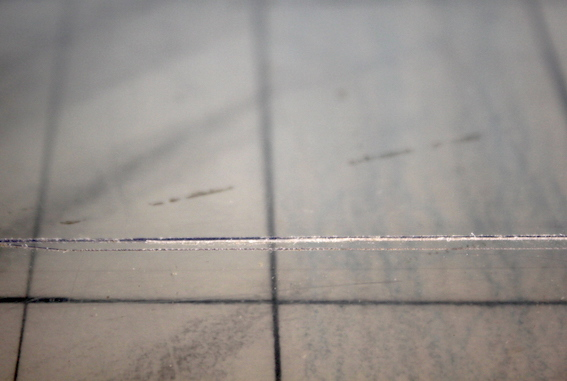
\includegraphics[width=\linewidth]{gfx/05_interfaces/Filigramophone_gravure_72dpi.jpg}
		\caption{Gravure d'une ligne médiane sur la plaque de \gls{PMMA}}
		\label{fig:interface:filigramophone-plexigravure}
	\end{minipage}
\end{figure}
%------------ Figure : filigramophone et xypre piezo -----------

\subsubsection{Repères dynamiques : fretting audiotactile}
\label{sec:audio-fretting}
\noindent Le déclenchement d'impulsion dans un haut-parleur tactile peut aider à sentir les paliers dans la progression d'un geste continu (e.g. les différentes ``notes'' d'une échelle de hauteur). Ce type de retour tactile fonctionne uniquement en réponse à un mouvement, le repère n'est pas sensible de manière statique. Son avantage par rapport à un repère physique (e.g. adhésif) .\\

Spatialisation ou diffusion ad-hoc
Travail avec Pascale Criton à la maison des aveugles

\subsubsection{Vérouillage des composants GUI}
\noindent Une solution logicielle partielle à ce problème et largement utilisée dans les systèmes de \gls{GUI} consiste à vérouiller l'interaction avec le composant GUI tant que le doigt est en contact avec la surface tactile, ce qui permet d'utiliser l'intégralité de l'écran tactile pour l'interaction et d'avoir des gestes plus amples. Ce solution nécessite toutefois que le composant ait bien été ciblé au moment du contact initial.




%%%%%%%%%%%%%%%%%%%%%%%%%%%%%%%%%%%%%%%%%
\section{Un exemple pratique : phylogenèse d'interfaces de type tablette}
\label{sec:interfaces:phylogenese}

\noindent Cette partie retrace le développement d'une série d'interfaces de \glspl{DMI}, basée sur un archétype d'instrument de type ``tablette''. On peut voir dans la tablette graphique des liens évidents avec les gestes du dessin et de l'écriture (todo: ref N d'Alessandro), tandis que l'écran multitouch possède certains liens avec les interactions nouvelles qui ont émergé avec les smartphones et autre tablette de type iPad.

Filigramophone : évolution depuis la tablette graphique simple, tablette augmentée, écran \textit{multitouch} augmenté, intégration de Bela…

De la simple tablette graphique à l’écran \textit{multitouch} augmenté de capteurs, histoire de l’évolution d’une interface pour la performance électroacoustique.
La conception d’une nouvelle interface pour la performance musicale est une tâche complexe, nécessitant de nombreux aller-retours entre conception, fabrication et pratique musicale. Le filigramophone est une interface qui a connu plusieurs versions, suffisamment différentes pour avoir envie de leur donner un nouveau nom à chaque fois et suffisamment similaire pour y voir la continuité d’un seul et même instrument.

%----------------------------------------------------------------------------------------------------------
\subsection{Origine : la tablette graphique (2005)}

TODO : rajouter un mot sur historique tablette (système UPIC de Iannis Xénakis, ou Fairlight CMI)

\noindent La tablette graphique (précisément un modèle Sapphire de Wacom) a été l’interface originelle qui a servi de base au filigramophone. J’ai commencé à l’utiliser dans le cadre du développement de la Méta-Mallette\footnote{Logiciel pour la pratique collective de musique par ordinateur développé par l’association Puce Muse, au développement duquel j'ai activement participé entre 2005 et 2008.}. Le choix de cette interface était motivé par la diversité de gestes expressifs possibles sur une tablette graphique, ainsi que par son coût relativement abordable\footnote{un peu moins de 100€ en 2005, autour de 50€ pour un modèle équivalent en 2019.} comparativement à la plupart des interfaces \gls{MIDI}, permettant de la déployer en nombre, dans le cadre d'activités pédagogiques pratiquées en groupe, dans des écoles et autres collectivités.\\
\indent En dehors de son usage pour la composition, un certain nombre de musiciens, compositeurs et concepteurs de \gls{NIME} l’ont par ailleurs adoptée pour la performance\footnote{Notamment à l'\gls{IRCAM} (voir \cite{wanderley_choice_2000}), au \gls{CNMAT} (voir \cite{zbyszynski_ten_2007}, au \gls{LMA} \cite{couturier_utilisation_2004}, au \gls{LIMSI} \cite{feugere_chorus_2011} puis dans l'équipe \gls{LAM} \cite{xiao_t-voks_2019}, mais on peut également citer Pierre Jodlowski (voir \url{https://youtu.be/pLARXmGwIO4}) ou Jesper Nordin (voir \url{https://gestrument.com/})}. Nicolas d’Alessandro a consacré une partie de son travail de thèse \cite{dalessandro_realtime_2009} à ce sujet, en proposant une étude détaillée des différentes échelles de mouvements dans le geste du dessin et de l'écriture, liées à l'articulation entre doigts, poignet et épaule.\\
\indent J'avais utilisé la tablette graphique pour différents projets\footnote{filigram, Media Music rooM, cf. \url{http://vincentgoudard.com}}, mais comme un composant parmi d'autres interfaces \gls{MIDI} ou de type joystick.
\indent Un des inconvénient de la tablette Wacom est que les contours de la surface utile, plus petite que la surface de la tablette\footnote{Cela permet de ne pas ``tomber'' hors de la tablette}, sont à peine perceptibles, tant visuellement qu'au niveau tactile. Cela s'avère problématique quand on manipule un processus sonore et non un pinceau dans PhotoShop, tel que l'usage de la tablette le prévoit. Une première adaptation a donc consisté à rajouter des bandes adhésives permettant de matérialiser cette frontière, visuellement et tactilement (cf. figure \ref{fig:interface:wacom}).\\
%-------------------------- Figure : wacom ---------
\begin{figure}[!htbp]
	\captionsetup{format=plain}%
	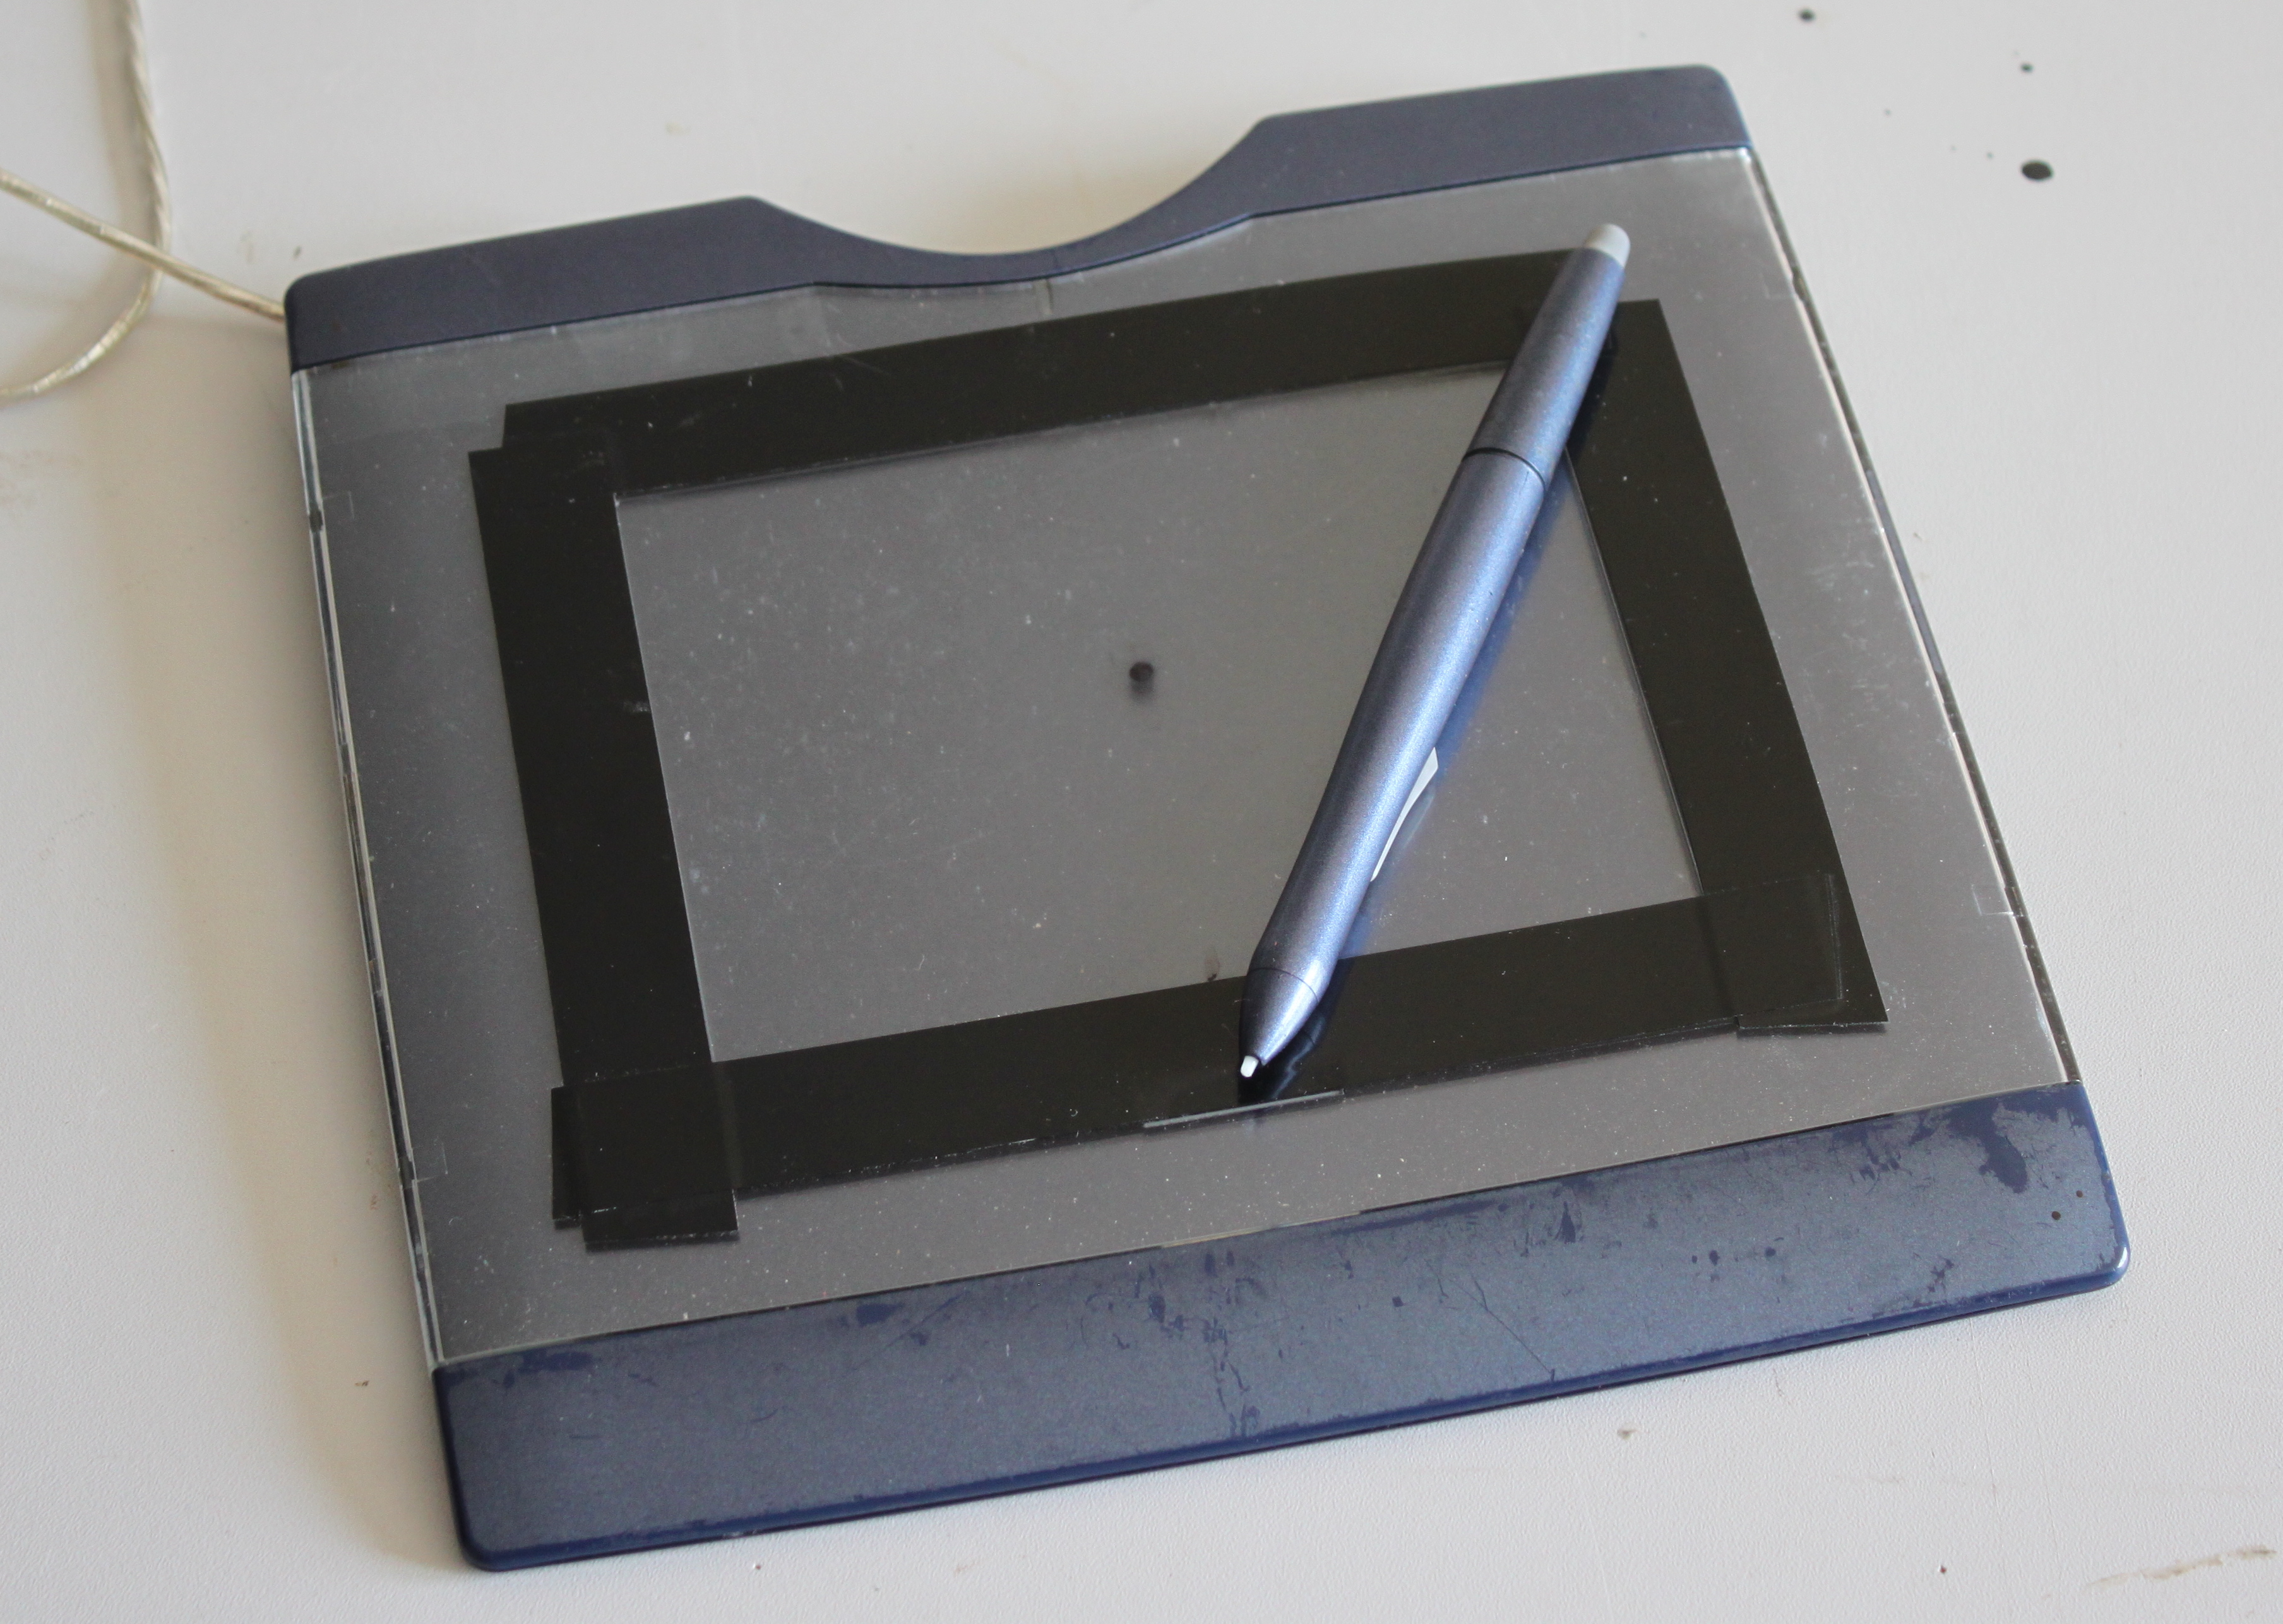
\includegraphics[width=\textwidth]{gfx/05_interfaces/wacom.jpg}
	\caption[Tablette wacom]{Tablette Wacom utilisée à l'origine. Des adhésifs rajoutés en bordure guident la perception haptique, un point central sert de repère visuel.}
	\label{fig:interface:wacom}
\end{figure}
%-------------------------- Figure : wacom ---------
\indent En 2007, dans l'équipe \gls{LAM}, Hugues Genevois avait acquis de nouveaux transducteurs tactiles large bande\footnote{Cette nouvelle génération offrait une bande passante de l'ordre du Hz jusqu'à plusieurs kHz, bien supérieure aux actuateurs linéaires, ainsi qu'une dynamique supérieure à celle des transducteurs piezo. Cette technologie a depuis équipé de nombreux cinéma pour transmettre une sensation plus tactile}. Nous avons fait l'expérience d'en placer un sous une tablette graphique, sur laquelle nous controlions la lecture d'un échantillon en se servant du stylet comme d'une tête de lecture virtuelle. La sensation haptique résultant était tout à fait saisissante et donnait l'impression que la surface de la tablette avait un relief similaire aux reliefs entendu dans le son : littéralement, l'impression de ``toucher le son''. Ce ``relief'' est bien entendu éphémère car ces transducteurs ne transmettent pas le continu et leur course est faible\footnote{ce qui les différencie nettement des systèmes de retours haptiques tels que développés, en particulier, à l'\gls{ACROE}}, mais la sensation est tout à fait confondante. J'ai donc utilisé ce système directement sur la tablette graphique, qui était une sorte de prototype du Filigramophone présenté ci-après.

%----------------------------------------------------
\subsection{Le Filigramophone: une tablette augmentée (2013)}

%-------------------------- Figure : filigramophone ----------------------------------
\begin{figure}[!htbp]
	\includegraphics[width=\textwidth]{gfx/filigramophone/filigramophone_overview.jpg}
	\caption{filigramophone - vue d'ensemble, débranchée}
	\label{fig:interface:filigramophone}
\end{figure}
%----------------------------------------------------------------------------------------------------------
\noindent L'expérience décrite précédemment a sucité le développement d'une interface plus intégrée, augmentant la tablette graphique d'une dimension acoustique bi-directionnelle, en captant d'une part le son de la tablette à l'aide de microphones piezo et en diffusant des signaux audio dans la tablette à l'aide de transducteurs tactiles.

\subsubsection{Intégration des microphones piezo}

\indent En effet, si la tablette graphique est une interface relativement expressive, par la possibilité qu'elle offre de contrôler trois, voire cinq variables continues en même temps\footnote{La position horizontale et verticale, la pression, et sur certains modèle, l'inclinaison du stylet selon les deux axes.}, sa fréquence d'échantillonage reste relativement faible\footnote{Généralement de 100Hz, d'après Wacom, mais l'objet wacom recevant les données de manière asynchrone dans Max ne permet pas la pleine exploitation de cette fréquence.} et la latence importante\footnote{La latence entre le mouvement du stylet et l'arrivée des données est de l'ordre de 50ms, alors qu'elle est de l'ordre de 5ms pour le \gls{MIDI}.}. Le désir de l'augmenter de microphones est ainsi largement lié à cette sensation de distance, qu'on retrouve de manière générale dans la plupart des interfaces de contrôle de type \gls{MIDI} (bien que moindre dans le \gls{MIDI}, cette distance est également sensible).\\
\indent Ali Momeni avait réalisé ce type d'augmentation acoustique, en plaçant un microphone piezo directement sur la tablette\footnote{Développements présentés dans sa thèse \cite{momeni_composing_2005}}. Cette technique lui permet de \iquote{Taper, gratter, frapper avec un anneau métallique ou frotter la tablette} pour obtenir une variété de signaux audio captés par le microphone piezo.\\
\indent Plus récemment, Romain Michon a étudié différentes possibilités d'effectuer des gestes percussifs et de pression sur une tablette \textit{multitouch}\footnote{Voir \cite{michon_nuance_2016}}, et proposé une solution hybride par l'ajout de capteurs \gls{FSR} placés sous un iPad, modulés en amplitude et récupérés via l'entrée audio d'un iPad. L'intérêt de cette solution est de permettre le calcul de la vélocité des gestes percussifs, en plus de l'aftertouch, mais la fusion des informations de pression et de coordonnées X/Y, bien que judicieusement contournée par une triangulation des différents \gls{FSR}, reste problématique comme le remarque son auteur. Par ailleurs, cette solution utilisant des capteurs de pression, sous la surface rigide de l'iPad ne permet pas d'exploiter la variation de hauteur spectrale en fonction du lieu de frappe, la surface de l'iPad étant trop rigide et les \gls{FSR} inadaptés à cette gamme de fréquences.\\
%------------ Figure : filigramophone et xypre piezo -----------
\begin{figure}[!htbp]
	\captionsetup{format=plain}%
	\centering
	\begin{minipage}[t]{0.48\textwidth}
		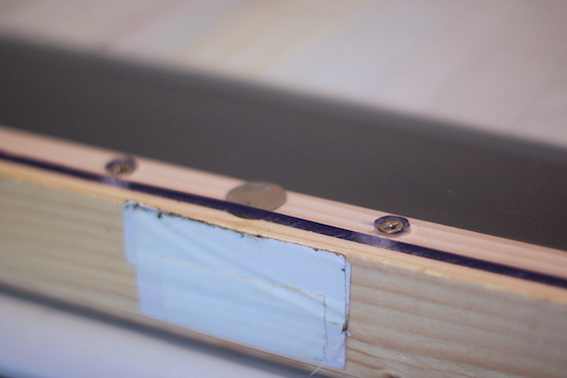
\includegraphics[width=\linewidth]{gfx/05_interfaces/filigramophone-piezo_72dpi.jpg}
		\caption{Transducteur piezo entre la vitre et le chassis sur le Filigramophone}
		\label{fig:interface:filigramophone-piezo}
	\end{minipage}
	\hspace{.02\linewidth}
	\begin{minipage}[t]{0.48\textwidth}
		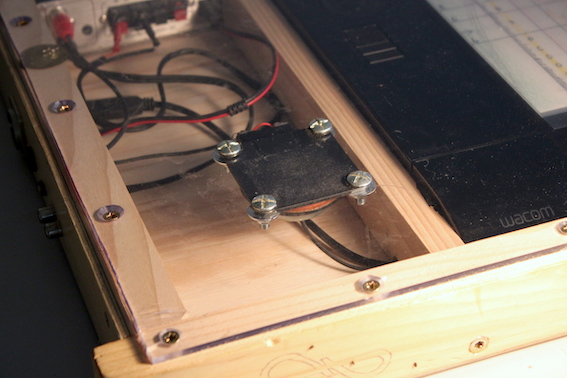
\includegraphics[width=\linewidth]{gfx/05_interfaces/filigramophone_hp_72dpi.jpg}
		\caption{HP tactile sur le Filigramophone}
		\label{fig:interface:filigramophone-hp}
	\end{minipage}
\end{figure}
%------------ Figure : filigramophone et xypre piezo -----------
\indent J'ai pour ma part choisi d'insérer les microphones piezo entre une vitre en \gls{PMMA} et le chassis contenant la tablette graphique (cf. figure \ref{fig:interface:filigramophone-piezo}). Cela permet des gestes percussifs, de frottements ou l'utilisation d'objet mis en mouvement (toupies, dés, diques, etc.) directement sur la surface, tout en conservant --~à travers le \gls{PMMA}~-- l'usage de la tablette qui renvoit les coordonnées horizontale et verticale ainsi que la pression et l'inclinaison du stylet. Ces transducteurs piezo permettent de capter les différents timbres de la surface \gls{PMMA}, qui présente une certaine élasticité (par rapport à la surface rigide de la tablette) en étant fixée uniquement sur ses bords, et dont la hauteur spectrale est plus grave au centre et plus aigüe sur les bords, à la manière d'une peau de tambour. Il est également possible de frapper sur le chassis, ce qui permet d'obtenir encore d'autres nuances de timbre (figure \ref{fig:interface:filigramophone-toupie}). Cette solution évite par ailleurs les bruits ``parasites'' de la structure de la tablette graphique quand on frappe directement dessus. Enfin, l'ajout de la plaque de \gls{PMMA} laisse la possibilité de dessiner, ajouter de l'adhésif, ou graver directement directement sur le \gls{PMMA} (tel que présenté dans la section \ref{todo}), sans déteriorer la tablette. Eventuellement, disposer de différentes plaques de \gls{PMMA} permettrait d'adapter l'interface à différentes configurations, à la manière des ce que permettent les \textit{overlays} sur les interfaces commerciales \textit{Joué} et \textit{SenselMorph}\footnote{\url{https://www.play-joue.com}, \url{https://sensel.com}}, ou à des compositions différentes, telles que les ``\textit{tangible scores}'' d'Enrique Tomás \cite{tomas_tangible_2014}.

%-------------------------- Figure : filigramophone-toupie ----------------------------------
\begin{figure}[!htbp]
	\captionsetup{format=plain}%
	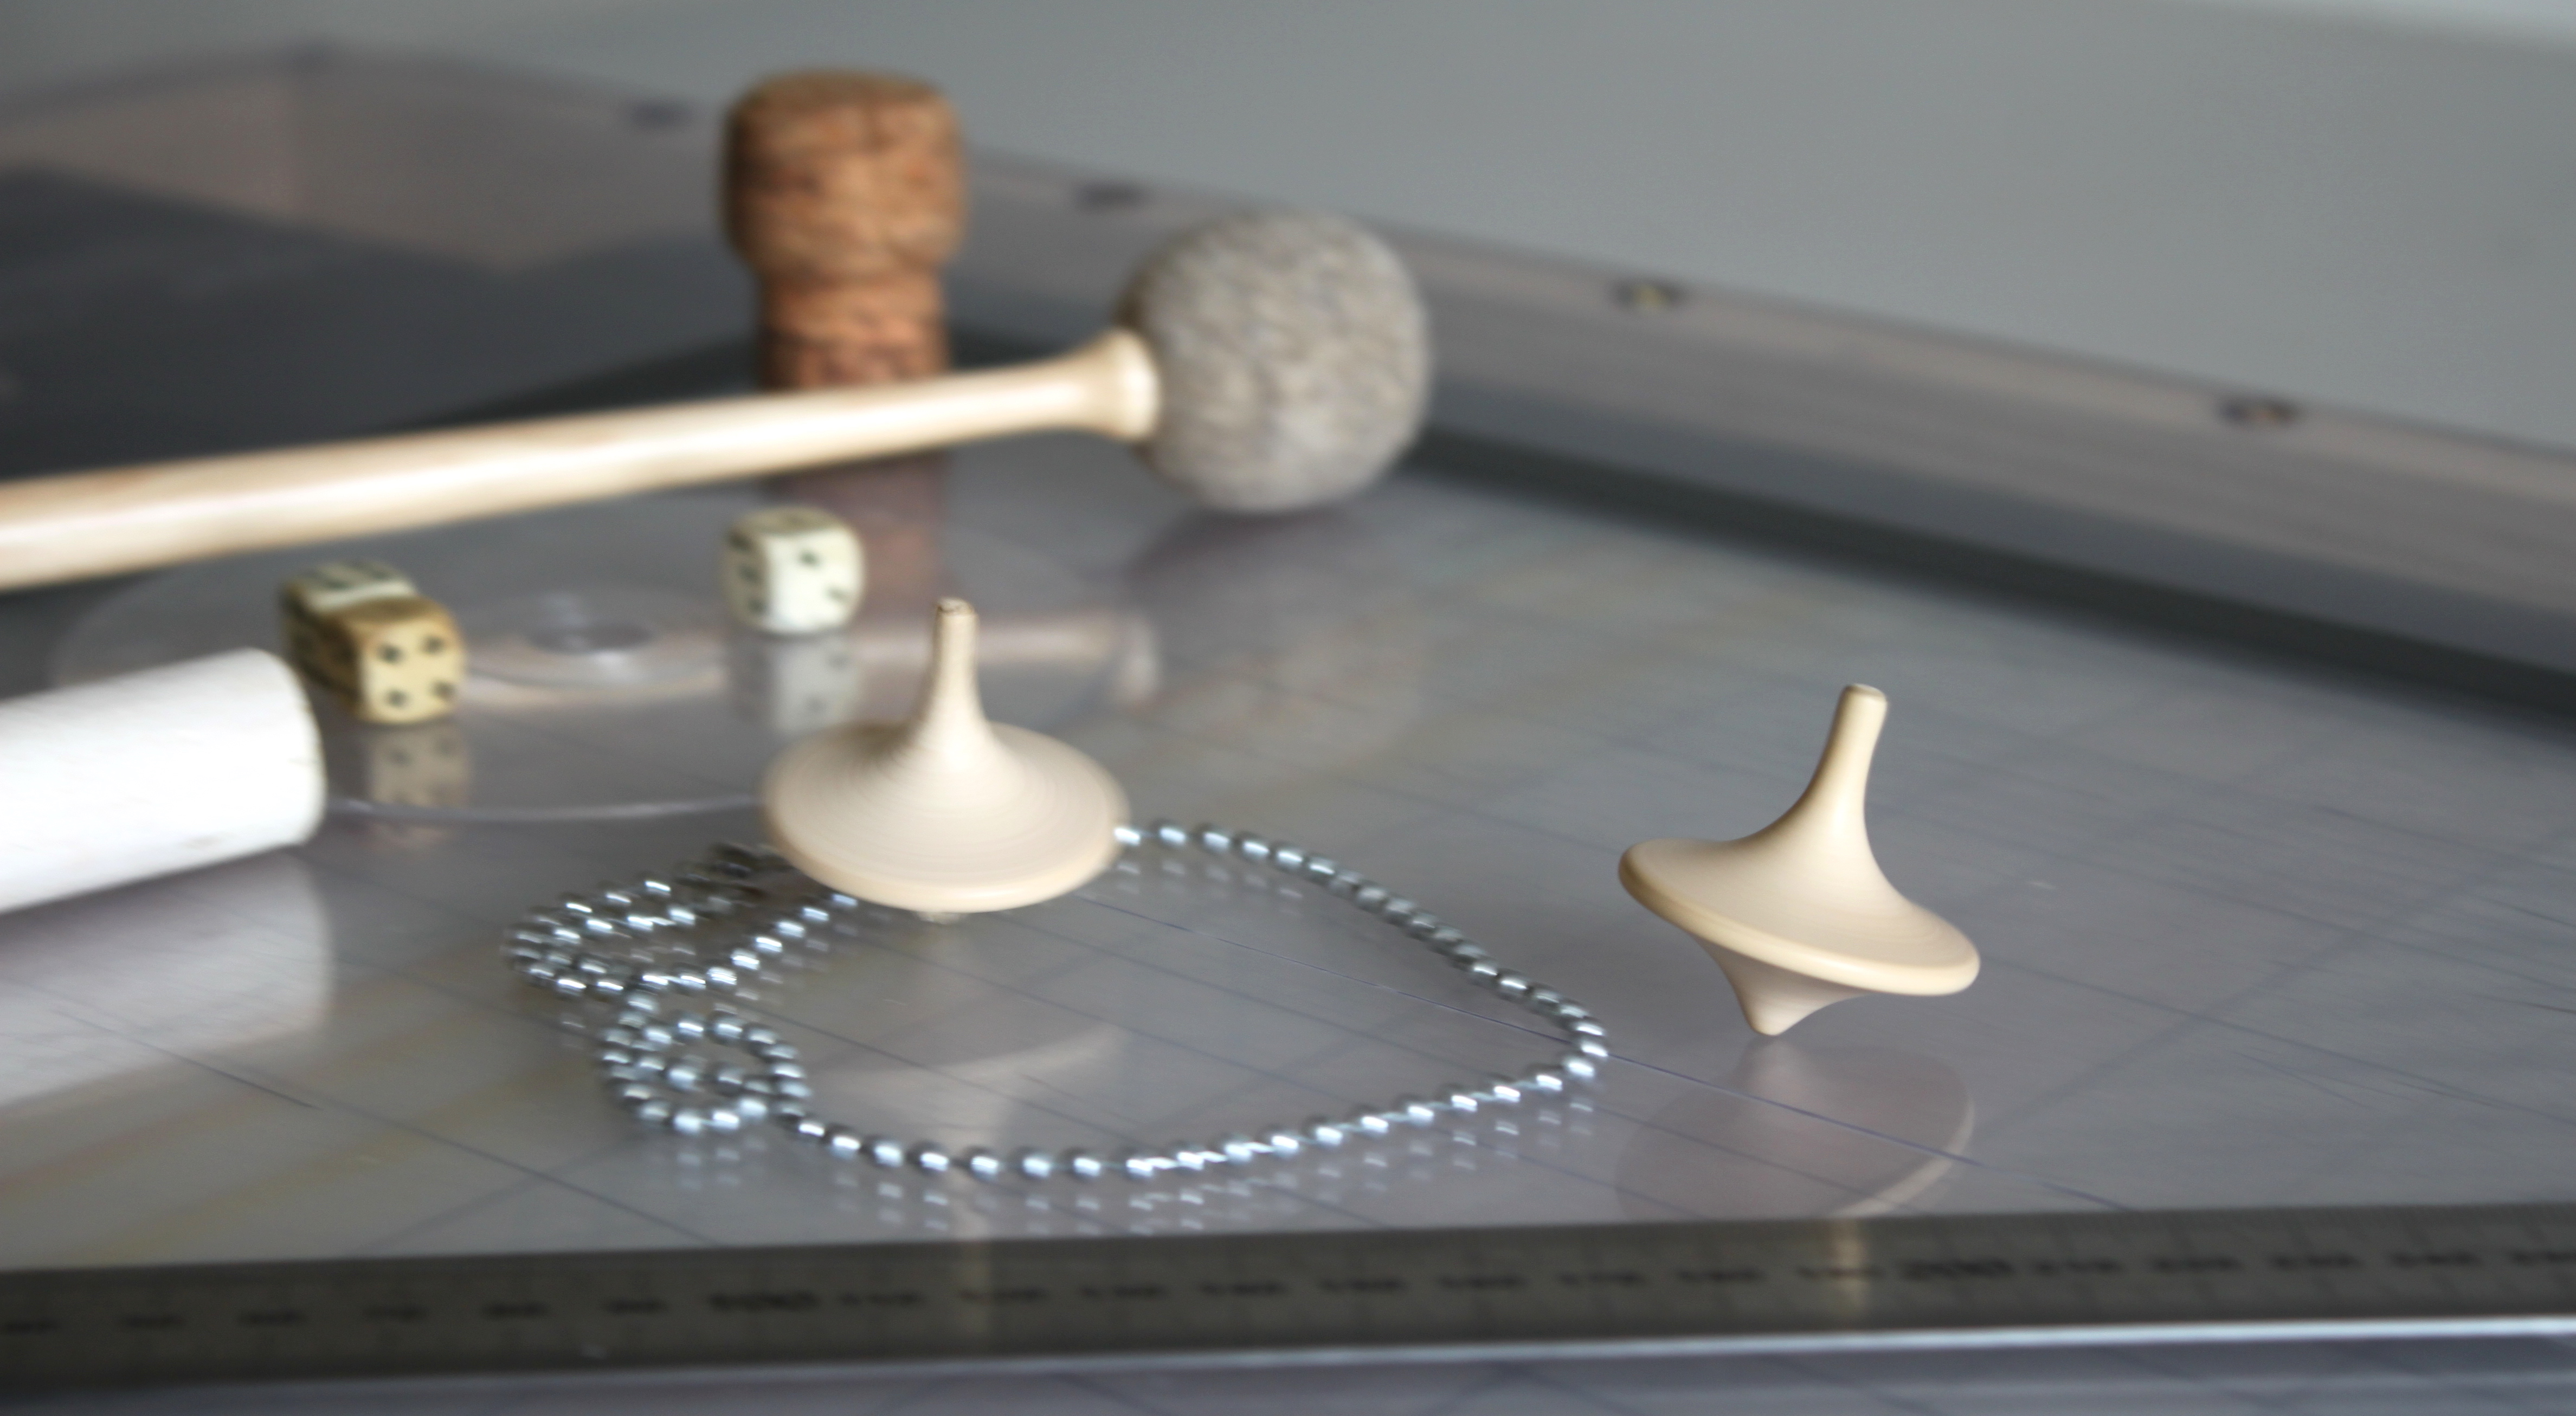
\includegraphics[width=\textwidth]{gfx/05_interfaces/filigramophone-toupie.jpg}
	\caption[Captation du son des mains ou d'objets sur la surface du Filigramophone]{Le microphone piezo laisse la possibilité de capter le son des mains ou d'objets sur la surface du Filigramophone}
	\label{fig:interface:filigramophone-toupie}
\end{figure}
%-------------------------- Figure : filigramophone-toupie ----------------------------------

\subsubsection{Intégration du transducteur tactile}

\noindent Parallèlement, un transducteur a été fixé sur la vitre de \gls{PMMA} (cf. figure \ref{fig:interface:filigramophone-hp}), et positionné empiriquement\footnote{C'est à dire, par un balayage des fréquences, envoyé sur le transducteur, en écoutant et en touchant la surface pour y trouver les zones de résonance.} pour favoriser l'excitation des premiers modes de résonance de la plaque de \gls{PMMA} sans être toutefois dans la zone d'interaction de la tablette graphique. Les premiers modes de résonance correspondent en effets aux fréquences les plus basses, et le but était ici d'avoir une vibration aussi forte que possible dans un domaine vibrotactile qui n'empiète pas trop sur le domaine audible.\\
\indent Le transducteur tactile est utilisé à la fois pour le retour vibratoire et la communication d'information, en particulier par frettage virtuel de la surface (cf. section \ref{todo}). Le retour vibratoire de l'instrument se distingue toutefois de l'envoi pur et simple du signal audio, la perception tactile ne lui étant pas directement liée. Au lieu de cela, un signal sinusoidal à 70Hz, correspondant à une fréquence de résonnance de la vitre de \gls{PMMA}, modulé par l'enveloppe du son final, ainsi que par sa dérivée spectrale, afin de mieux sentir dans les doigts les transitions et les ruptures du son (cf. figure TODO : schéma de principe du patch / développement dans une autre partie ?).\\
\indent Le Filigramophone a été joué plusieurs fois en concert, à la fois dans l'ensemble ONE, ainsi que dans la première version de la performance audio-visuelle ``FIB\_R'' avec la plasticienne Gladys Brégeon (cf. figure \ref{fig:interface:filigramophone-Xypre-Triton}). Le dispositif complet était composé du Filigramophone, d'un ordinateur faisant tourner un patch Max pour la synthèse, d'une carte son et haut-parleurs, ainsi que d'une interface \gls{MIDI} Akai MPD24, donnant un accès direct à davantage de paramètres tels que le volume général, le mixage entre différentes synthèses, le rappel de configurations, la sélection d'échelles musicales pour l'accordage, ainsi que divers autres paramètres spécifiques aux algorithmes de synthèse.

%-------------------------- Figure : fibroscopie Triton ----------------------------------
\begin{figure}[!htbp]
	\captionsetup{format=plain}%
	\includegraphics[width=\textwidth]{gfx/05_interfaces/fibroscopie-Triton.jpg}
	\caption{Filigramophone (à droite) et une version protoypique du Xypre v1 (à gauche) sur scène, durant la répétition de la première de FIB\_R en juin 2015, Le Triton, Les Lilas (93)}
	\label{fig:interface:filigramophone-Xypre-Triton}
\end{figure}
%-------------------------- Figure : fibroscopie Triton ----------------------------------


%---------------------------------------------------------------
\subsection{Xypre : écran multitouch augmenté (2015, 2018)}
%------------ Figure : xypre - plan et vue d'ensemble -----------
\begin{figure}[!htbp]
	\captionsetup{format=plain}%
	\centering
	\begin{minipage}[t]{0.365\textwidth}
		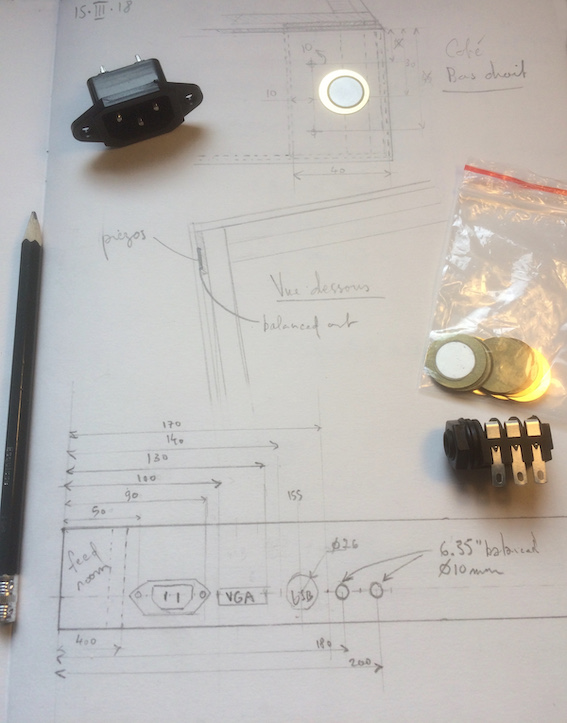
\includegraphics[width=\linewidth]{gfx/05_interfaces/Xypre_plan01_72dpi.jpg}
		\caption{Xypre v2 - plans de conception}
		\label{fig:interface:xypre_plans}
	\end{minipage}
	\hspace{.01\linewidth}
	\begin{minipage}[t]{0.6\textwidth}
	    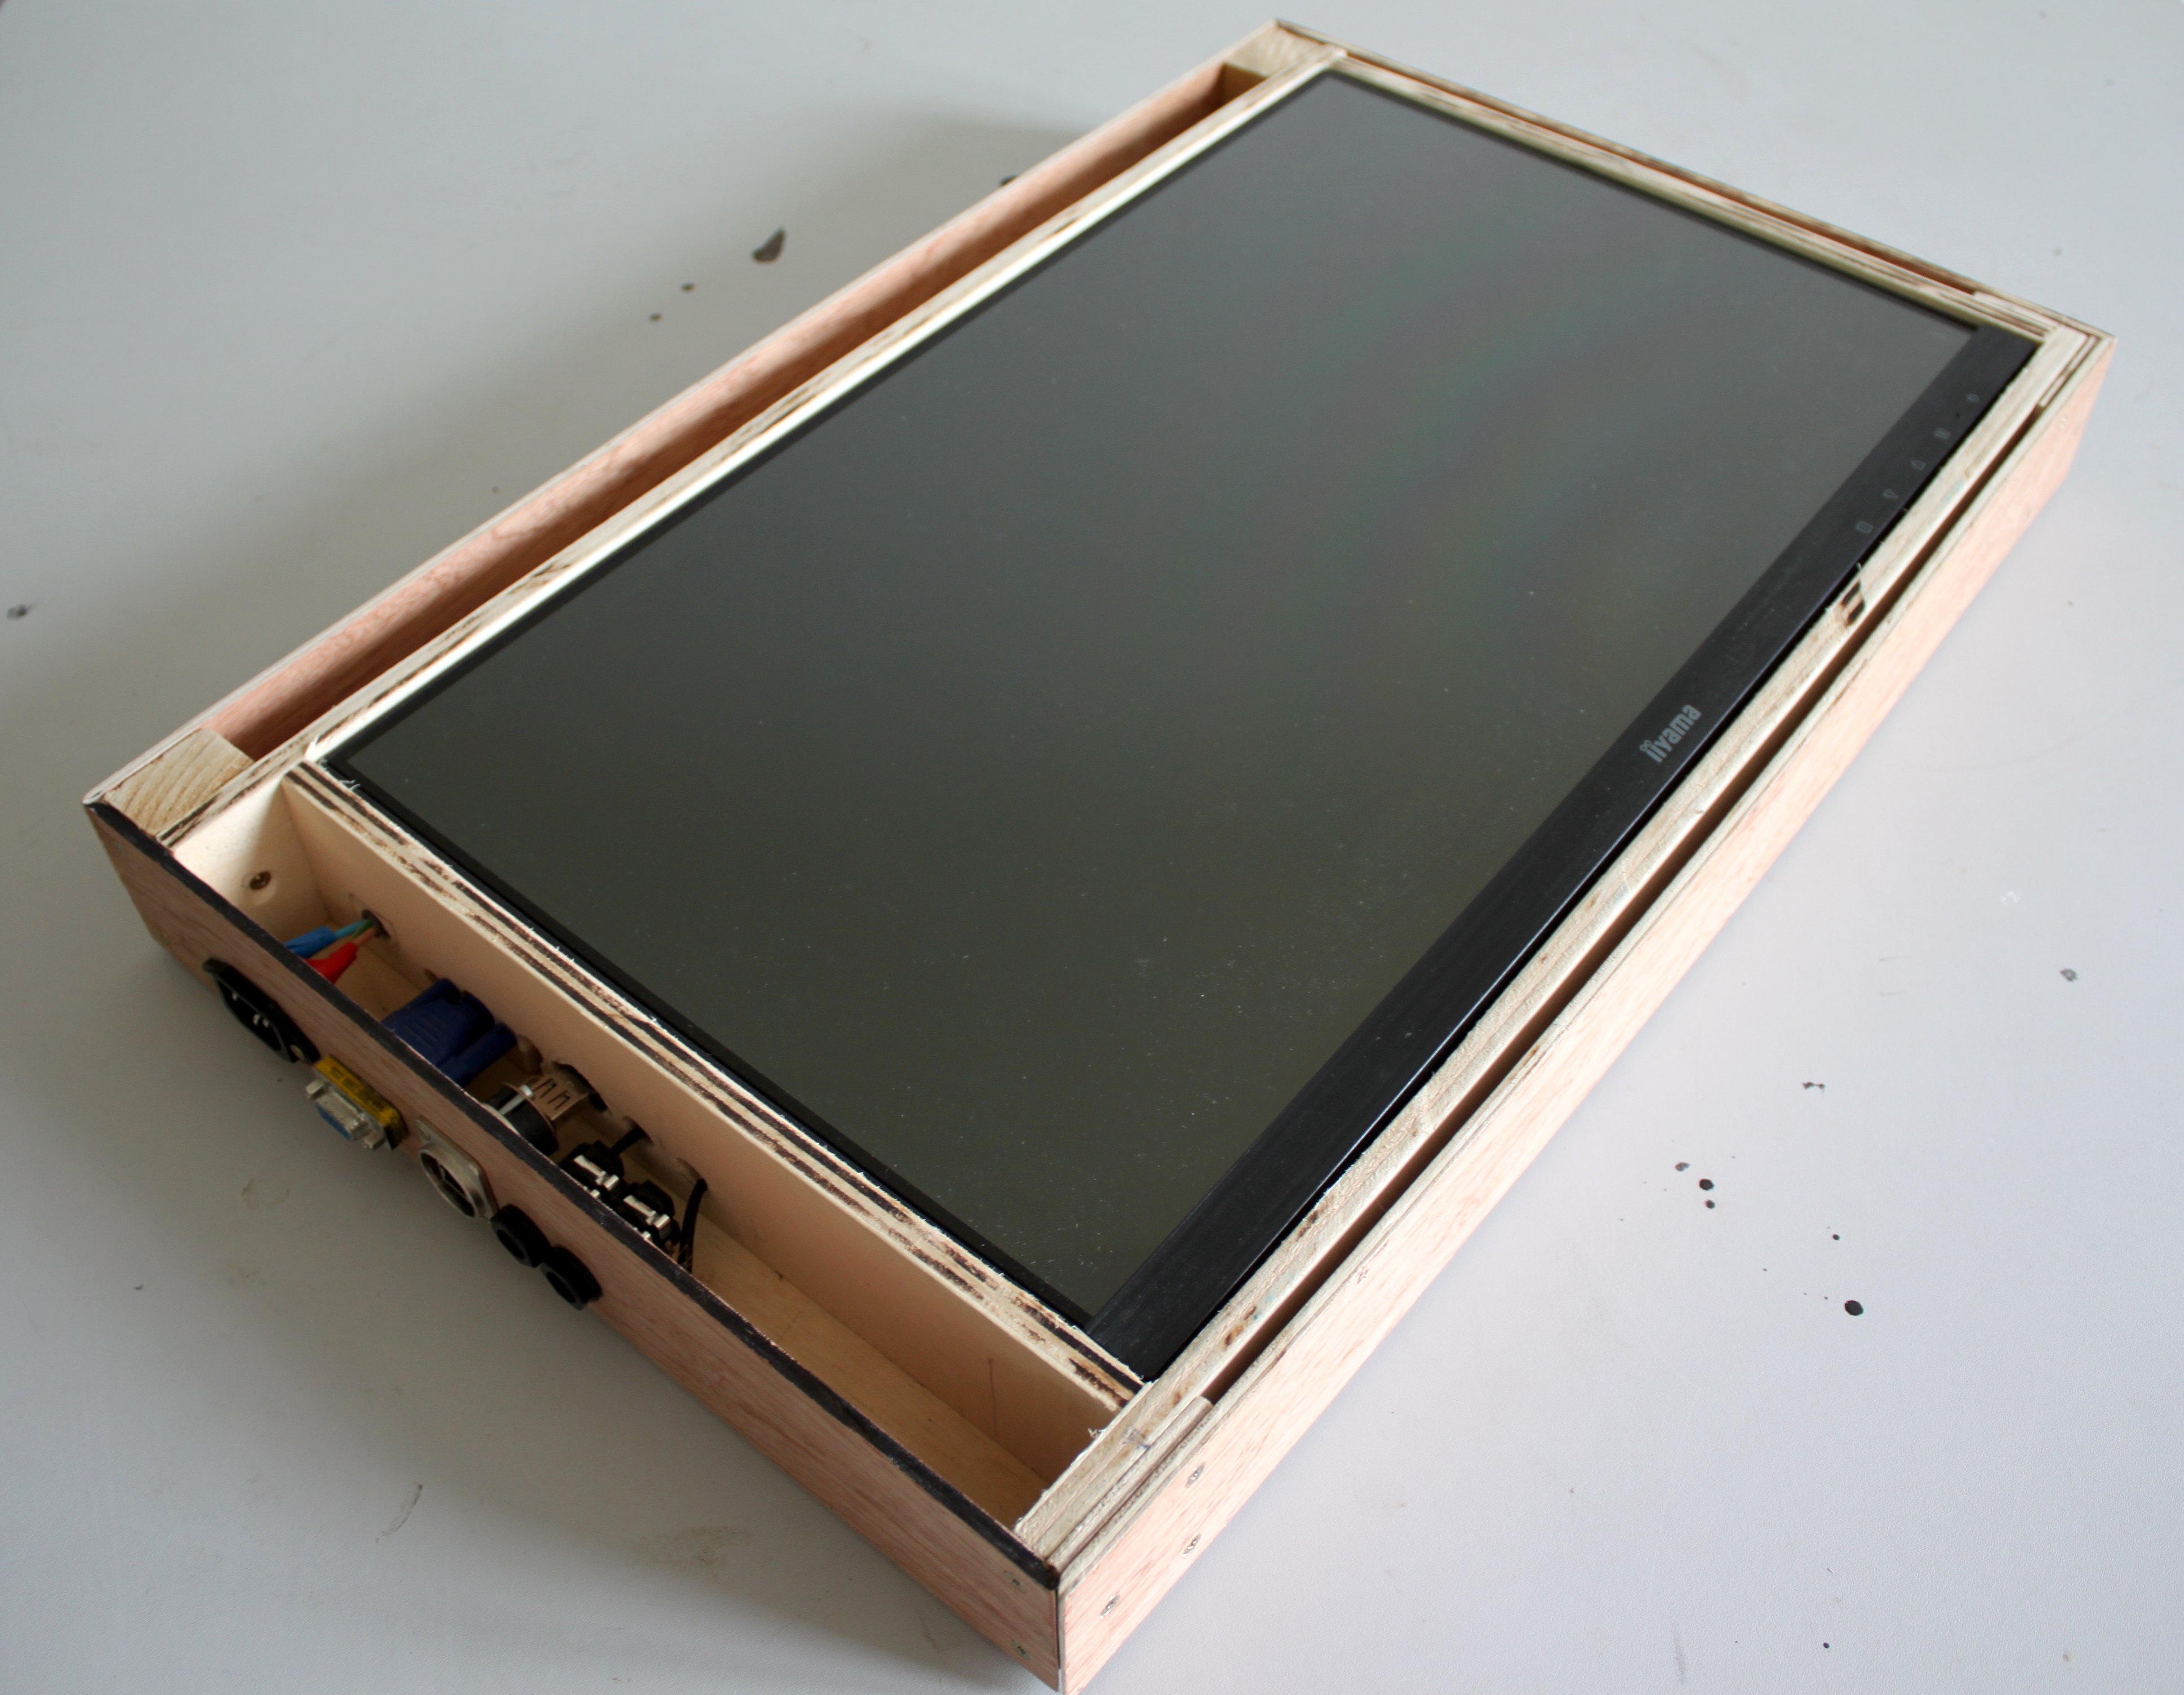
\includegraphics[width=\linewidth]{gfx/05_interfaces/xypre_overview_unplugged.jpg}
		\caption{Xypre - vue d'ensemble, débranchée}
		\label{fig:interface:xypre}
	\end{minipage}
\end{figure}
%------------ Figure : xypre - plan et vue d'ensemble -----------

\noindent L'utilisation du Filigramophone lors de performances musicales a permi de constater plusieurs points d'améliorations possibles, qui ont donné lieu au développement d'une nouvelle interface, nommée Xypre\footnote{Une vidéo montre en accéléré le processus de fabrication de la version 2 du Xypre : \url{https://vimeo.com/358401223}}:
\vspace{-1em}
\begin{itemize}[noitemsep]
	\item La taille de l'interface le rendait intransportable en avion en tant que bagage cabine, et de manière plus courante, peu pratique dans le métro parisien;
	\item Son poids rendait également son transport pénible, malgé une pochette à dessin adaptée\footnote{Un avantage d'un tel format ``tablette'' est qu'il est relativement facile de trouver des sacs d'artiste, habituellement destinés au transport de dessins, dans un grand nombre de formats.}. Notamment le chassis, trop massif, pouvait être allégé;
	\item La nécessité d'une interface complémentaire (le MPD24) augmentait d'autant le temps de montage, de démontage, ainsi que le poids global;
	\item La relative fixité des repères visuels sur le calque de la tablette, qui exigeaient un démontage fastidieux pour être changées, et qui du coup, ne l'étaient pas;
	\item Le jeu polyphonique y était limité, tant par l'unicité du stylet que par l'absence de retour visuel permettant de gérer différentes couches de manière indépendante avec un seul stylet.
\end{itemize}

\noindent Le poids et la taille ont été diminués en utilisant du contreplaqué plus fins pour le chassis et en adoptant un format de valise cabine, offrant une surface équivalente à la surface utile de la tablette graphique utilisée dans le filigramophone, suffisamment large --~quoique juste assez~-- pour permettre des gestes amples impliquant tout le bras.\\
\indent La solution adoptée pour les autres problèmes évoqués a consisté à remplacer la tablette graphique par un écran \textit{multitouch}, toujours augmenté de piezo et transducteurs tactiles, le retour visuel offert par les écrans permettant de virtualiser les contrôleurs physiques utilisés sur l'interface \gls{MIDI} MPD24\footnote{Voir la librairie graphique ``mp.TUI'' développée à cette fin et présentée au chapitre \ref{ch:visual_representation}}.\\
\indent Deux versions du Xypre ont été développées sur ce même principe, mais utilisant deux technologies différentes en ce qui concerne la captation \textit{multitouch} : l'une basée sur la détection par infra-rouge\footnote{Le modèle \textit{G4S-overlay} de la marque PQ-Labs (\url{https://www.pqlabs.com}) permettant théoriquement jusqu'à 32 points de contact simultanément} et l'autre sur une détection capacitive\footnote{Un écran tactile \textit{Iiyama ProLite T2252MSC}, intégrant une technologie ``capacitive projetée'' permettant la détection de dix points de contact simultanément.}. Les deux interfaces communiquant avec Max via le protocole \gls{TUIO}\footnote{A la différence, toutefois, que le G4S envoit directement des données \gls{TUIO} exploitables dans Max, alors que l'écran capactitif davantage destiné à un usage grand public ne les renvoit pas. Un driver payant, développé par la société \textit{Touch-Base Ltd.} est nécessaire pour convertir les données au format \gls{TUIO}.}, peu d'adaptations ont été nécessaires sur le patch Max gérant l'interaction et la synthèse audio. Toutefois, cette différence de technologie a des conséquences sur l'assemblage et sur les modes de jeu possibles. 

\subsubsection{Technologie multitouch et incidence sur le jeu}

\indent La technologie infra-rouge de l'\textit{overlay G4S} laisse la possibilité de poser des objets sur la surface, qui soient détectés par les capteurs infra-rouge. Cela permet notamment de pouvoir maintenir des processus actifs, par la présence physique d'objets (comme on maintiendrait une note enfoncée sur un orgue à l'aide d'un poids). Un inconvénient de cette technologie est la détection possible des doigts (ou d'objets) entrant dans le plan de détection, situé légèrement au-dessus de la surface de la vitre. Cela requiert par exemple de lever les doigts qui ne jouent pas relativement haut afin qu'il ne soit pas détectés par erreur, et provoque une tension musculaire pénible de la main.Egalement, cette technologie est plus sensible à la poussière qui peut provoquer de fausses détections.

\indent A l'inverse de la technologie infra-rouge, le capacitif ne détecte que la présence des doigts et pas celle d'objet quelconques. Il est possible de détecter la présence d'objets dédiés, intégrant un système électrique actif ou passif, stimulant le champ électrostatique de l'écran, ainsi que de reconnaître ces objets à l'aide d'identifiant spatiaux et/ou temporels\footnote{voir notamment \cite{rekimoto_datatiles_2001, yu_tuic_2011}}. Ce type de solution a notamment été utilisé dans l'application \textit{Rotor} de \textit{ReacTable}. Cette solution présente néanmoins l'inconvénient de nécessiter un circuit électronique dédié d'une part, et d'autre part la reconnaissance de l'objet consomme rapidement le nombre de point de contact détectable par l'interface\footnote{Par exemple, la détection de la position et de l'orientation nécessite généralement trois points de contact, ce qui signifie qu'un écran multitouch permettant dix points de contact ne pourra pas détecter plus de trois objets (et un doigt).}, en même temps qu'elle rajoute une latence due à l'analyse du motif déterminé par les points.

\subsubsection{Implantation des microphones piezo et transducteur tactile}
%------------ Figure : xypre piezo et HP -----------
\begin{figure}[!htbp]
	\captionsetup{format=plain}%
	\centering
	\begin{minipage}[t]{0.48\textwidth}
	    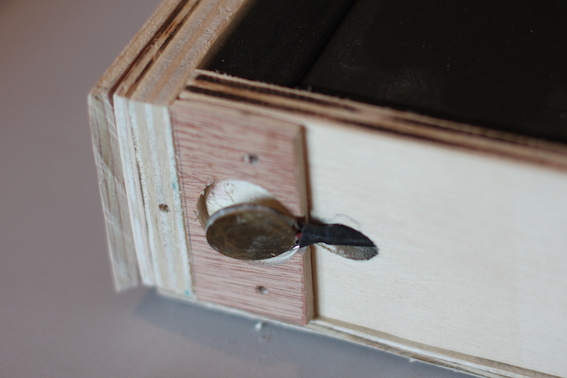
\includegraphics[width=\linewidth]{gfx/05_interfaces/xypre-piezo_72dpi.jpg}
		\caption{Transducteur piezo pseudo-symétrique dans le côté du chassis sur le Xypre v2 (plaque extérieur démontée)}
		\label{fig:interface:xypre_v2-piezo1}
	\end{minipage}
	\hspace{.02\linewidth}
	\begin{minipage}[t]{0.48\textwidth}
	    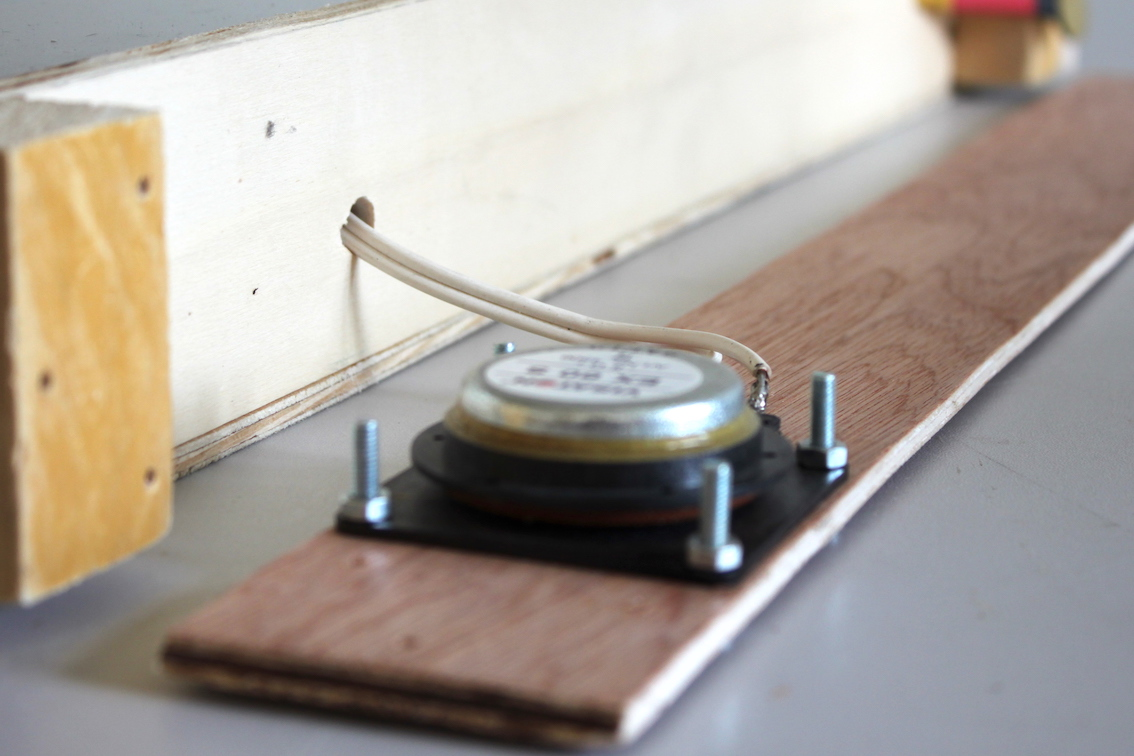
\includegraphics[width=\linewidth]{gfx/05_interfaces/Xypre_HP_144dpi.jpg}
		\caption{HP tactile sur le Xypre}
		\label{fig:interface:xypre_v2-hp}
	\end{minipage}
\end{figure}
%------------ Figure : xypre piezo et HP -----------

\indent \textbf{Sur le Xypre v1}, la technologie infra-rouge du cadre de détection du \textit{multitouch} permet d'insérer une vitre en \gls{PMMA} (cf. figure \ref{fig:interface:PQlabs-G4overlay}), pour un fonctionnement similaire à celui développé sur le Filigramophone. L'inconvénient qui résulte des gestes de percussion sur cette vitre est la transmission des vibrations au cadre de détection \textit{multitouch} et les bruits de plastique parasites qu'elles provoquent. Il serait envisageable de supprimer ces bruits en serrant le cadre multitouch entre des mousses, mais cet assemblage plus complexe n'a pas encore été testé.

\indent \textbf{Sur le Xypre v2}, l'écran \textit{multitouch} capacitif ne permettant pas l'ajout d'une vitre \gls{PMMA}, les microphones piezo ont été placées sur le côté du chassis, pré-contraints entre le chassis et une plaque de bois plus fine servant de surface de percussion. Cette plaque fixée sur deux côtés au chassis permet là-encore de récupérer différentes nuances de hauteur spectrale, utilisée pour la synthèse en aval (cf. figure \ref{fig:interface:xypre_v2-piezo1}). La pré-contrainte du piezo est en partie dûe à l'orientation verticale du piezo (qui chuterait, autrement) mais permet également d'utiliser une technique de pseudo-symétrisation du signal du piezo (cf. schéma fonctionnel figure \ref{fig:interface:balancedPiezo} et aperçu figure \ref{fig:interface:xypre_v2-piezo1}), qui s'avère très utile quand les transducteurs piezo sont utilisés à proximité d'un écran, source de perturbations électromagnétiques.\\
%-------------------------- Figure : balanced piezo ----------------------------------
\begin{figure}[!htbp]
	\captionsetup{format=plain}%
	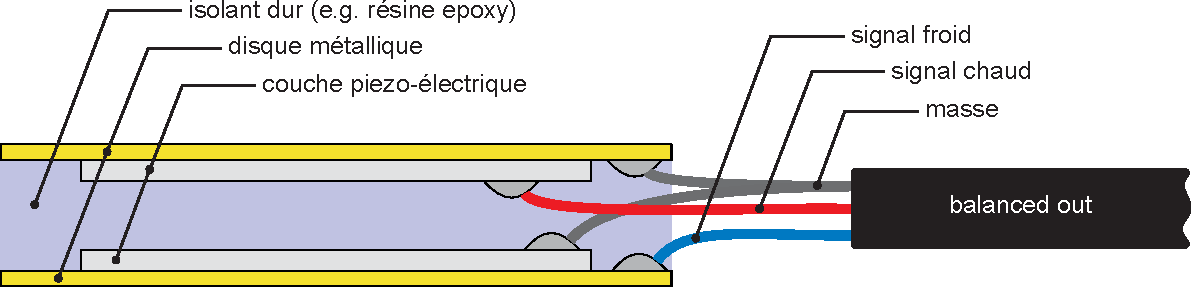
\includegraphics[width=\textwidth]{gfx/05_interfaces/balancedPiezo.pdf}
	\caption{Montage pseudo-symétrique de transducteurs piezo-électriques}
	\label{fig:interface:balancedPiezo}
\end{figure}
%-------------------------- Figure : balanced piezo ----------------------------------
\indent La séparation entre la surface percussive et l'interface \textit{multitouch} de l'écran a conduit à placer le haut-parleur tactile sur une plaque de contreplaqué à l'avant du chassis (cf. figure \ref{fig:interface:xypre_v2-hp}). Il se trouve ainsi relié acoustiquement au transducteur piezo \#2 (cf. figure \ref{fig:interface:xypre_v2-hppiezo}), tandis que l'autre transducteur (figure \ref{fig:interface:xypre_v2-piezo1}) est (relativement) isolé acoustiquement en étant positionné orthogonalement.

%-------------------------- Figure : xypre HP et piezo ----------------------------------
\begin{figure}[!htbp]
	\captionsetup{format=plain}%
	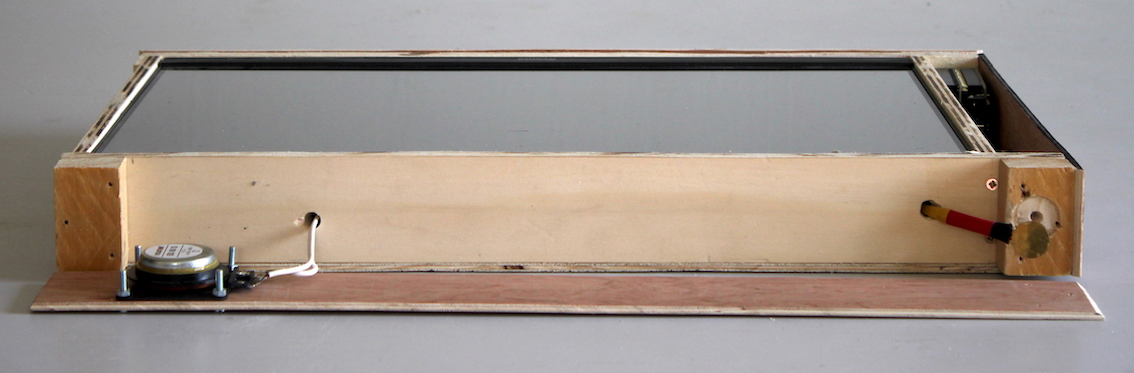
\includegraphics[width=\textwidth]{gfx/05_interfaces/Xypre_FrontPanel_144dpi.jpg}
	\caption{Liaison acoustique entre piezo et haut-parleur tactile sur le Xypre}
	\label{fig:interface:xypre_v2-hppiezo}
\end{figure}
%-------------------------- Figure : xypre HP et piezo ----------------------------------


%-------------------------- Figure : xypre ----------------------------------
\begin{figure}[!htbp]
	\captionsetup{format=plain}%
	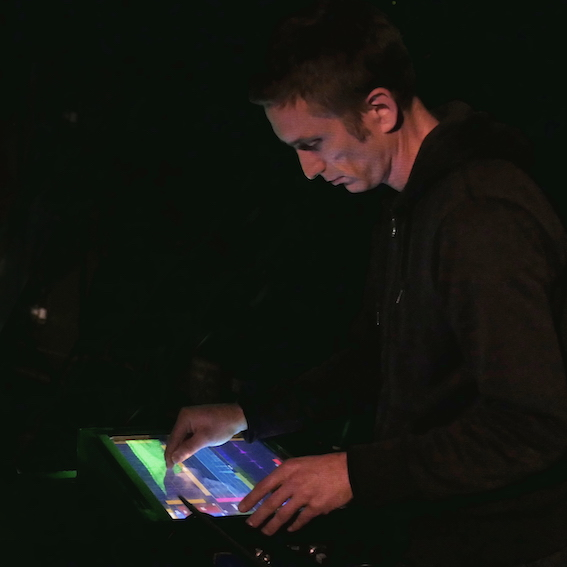
\includegraphics[width=\textwidth]{gfx/05_interfaces/xypre-v1_72dpi.jpg}
	\caption{Xypre v1 inauguré durant une performance avec ONE}
	\label{fig:interface:xyprev1_jeu}
\end{figure}


\subsection{Bilan et perspectives}

\noindent Si les interfaces multitouch conservent une parenté avec les tablettes graphiques, elles offre de nouvelles possibilités en même temps qu'elle impose d'autres contraintes. En particulier, la perte de la pression du stylet comme paramètre expressif est difficile à compenser et à distribuer dans d'autres gestes sans revoir considérablement le design d'interaction en aval. Il est tout de même prévu de rajouter des capteurs de type \gls{FSR} et capteurs de distance, d'une granularité temporelle et d'une expressivité intermédiaire entre celle permise par les microphones et celle permise par l'écran tactile.\\
\indent Une autre direction de développement (en cours), est l'autonomisation progressive de l'interface, en transférant le calcul de la synthèse audio et graphique depuis l'ordinateur sur lequel il tourne maintenant, vers des nano-ordinateurs tels que Raspberry Pi et Bela\footnote{\url{https://raspberrypi.org}, \url{https://bela.io}.}, tout en conservant une extension possible par l'ordinateur.\\
\indent Enfin, au niveau acoustique, l'usage de plaque de bois massive et/ou de métal est envisagé afin d'améliorer la liaison acoustique entre le microphone piezo et le transducteur tactile en façade. Si les premiers tests révelent des interactions intéressantes sur le contrôle du feedback (qu'on espère améliorer en utilisant une carte Bela à très faible latence), le contreplaqué semble un matériau trop épais et absorbant pour que des pressions directe sur la plaque interagissent efficacement avec la boucle de \textit{feedback}.

%%%%%%%%%%%%%%%%%%%%%%%%%%%%%%%%%%%%%%%%%

\section{Conclusion}
\label{sec:interfaces:conclusion}

Les DMIs ne sont pas purement virtuels: poids, encombrement, affordance, part acoustique, sensibilité, temps de montage.

Les interfaces hardware sont des objets auxquels on s'attache, plus que le virtuel (cf. Dumeaux, Dallio). Rapport sensuel.

Compromis entre modularité et intégration ergonomique.

Possibiltés offerte par le DIY avec les nouvelles cartes barebone (Ino, raspi, bela, etc.)

La question de l'acoustique, de l'haptique, de l'électronique et du numérique sont interdépendantes.







\section*{extra material}

\iquote{Though there is a huge range of performer decision, history, and knowledge that will determine their exact method of playing (as established by Jorda [12]), the physical design of the DMI impacts this gesture repertoire by presenting certain affordances.} \cite{bin_hands_2017}

\vspace{-1em}
\begin{itemize}[noitemsep]
\item Faire évoluer une interface en la raffinant (De Laubier, VG).
\item Faire évoluer une interface en rajoutant des choses (Patricia Dallio)
\item Faire évoluer en supprimant des choses (Dumaux)
\item Partir de l'objet (Patrick Saint Denis)
\end{itemize}

